%\documentclass[11pt, twoside, titlepage, a4paper, openright]{report}
\documentclass[12pt, titlepage, a4paper]{book}
\usepackage{graphicx}
\usepackage[english]{babel}
\usepackage[utf8]{inputenc}
\usepackage{algpseudocode}
\usepackage{amsthm}
\usepackage{algorithm}
\usepackage{rotating}
\usepackage{enumerate}
%\usepackage[Lenny]{fncychap}
\usepackage{hyperref}
\hypersetup{
    colorlinks=true,       % false: boxed links; true: colored links
    linkcolor=black,%red,          % color of internal links
    citecolor=black,%green,        % color of links to bibliography
    filecolor=black,%magenta,      % color of file links
    urlcolor=black%cyan           % color of external links
}
% \usepackage [a4paper,left=2.5cm,bottom=2.5cm,right=2.5cm,top=3cm]{geometry}
\usepackage{frontespizio}
\linespread{1.2}
\newtheorem{mydef}{Definition} % definizioni <-----
\usepackage{listings}
\lstset{
	language=C++,
	basicstyle=\small\ttfamily, 
	numbers=left,
	numberstyle=\tiny,
	frame=tb,
	columns=fullflexible,
	showstringspaces=false
}
\usepackage{multicol}
% \usepackage[style=numeric]{biblatex}
% \usepackage{multicol}

%\nofiles 
%\fontoptionnormal 
\usepackage{mathtools}

\frenchspacing

\newcommand{\srst}[0]{SR:ST\space}
\newcommand{\gsp}[0]{GSP1:N\space}
\newcommand{\sps}[0]{SPS1:N\space}
\newcommand{\mrs}[0]{MRS\space}
\begin{document}


\begin{frontespizio}
\Universita {Verona}
\Dipartimento {Informatica}
\Corso {Ingegneria e Scienze Informatiche}
\Annoaccademico {2017-2018}
\Titoletto {Tesi di Laurea Magistrale}
\Titolo { \Large {Multi-Robot Task Allocation for logistic applications} }
\Candidato [vr414572]{Davide Zorzi}
\Relatore {Alessandro Farinelli}
\Rientro {1.5cm}
\NCandidato {Candidato}
\end{frontespizio}

%\clearpage\null\thispagestyle{plain}\clearpage
%\newpage

%\preparefrontpage

% \bibliographystyle{unsrt}
% \bibliography{sample}

\tableofcontents

\newpage

\paragraph{Abstract}
\begin*{}
\newline
\newline
Robotics technology has recently matured sufficiently to deploy autonomous
robotic systems for daily use in several applications: from disaster response
to environmental monitoring and logistics.
In this project present and evaluate the principal difference of central and 
distributed allocator task coordinator. 
In these applications we address off-line coordination, by casting the Multi-Robot
logistics problem as a task assignment problem and proposing two solution 
techniques: Cyclic Greedy Strategy Single Robot Single Task (CGS1:1), which is 
a baseline greedy approach, and Cyclic Greedy Strategy Single Robot Multiple Task 
(CGS1:N), which is based on merging task for improve the spend time.
\\
And the last one is address on-line coordiantor, that is based on token passing (TP) approach.
We evaluate the performance of our system in a realistic simulation enviroment
(build with ROS and stage). In particular, in the simulated enviroment we compare
our task assignment approaches with previous off-line and on-line methods.
\newline
\newline
\textbf{Keywords:} Multi-Robot Task Allocator, logistic applications, Multi-Robot
systems, coordination, task assignment

% TODO: primi risultati e considierazioni

\end*{}




\chapter{Introduction}\label{chap:intro}

    \begin{frame}[fragile]{Industrial Logistics}
        The {\bf industrial logistics} is the process of {\bf planning}, {\bf organization}
        and {\bf control} of all the activities of handling and {\bf storage} of goods, which, starting
        from the suppliers and reaching up to the end user, guarantee an adequate
        level of {\bf service} to the customer consistent with the {\bf costs} to it associated

        \begin{figure}[hbt]
            \centering
            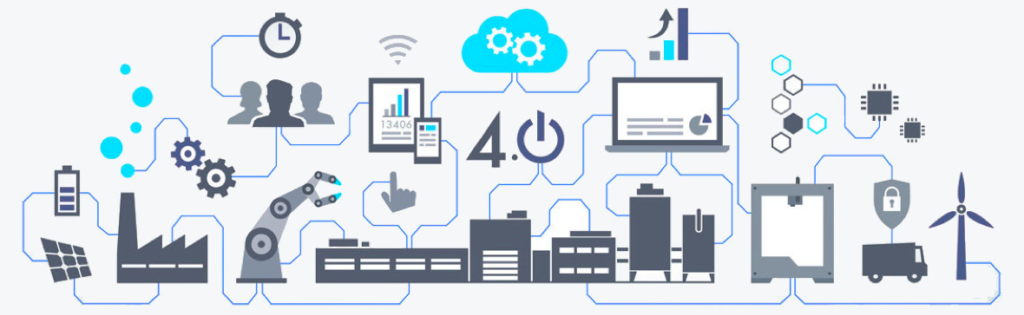
\includegraphics[width=\textwidth]{img/ind4.png}
        \end{figure}
    \end{frame}

    \begin{frame}[fragile]{Multi-Robot Systems for logistic applications}

        \begin{figure}[hbt]
            \centering
            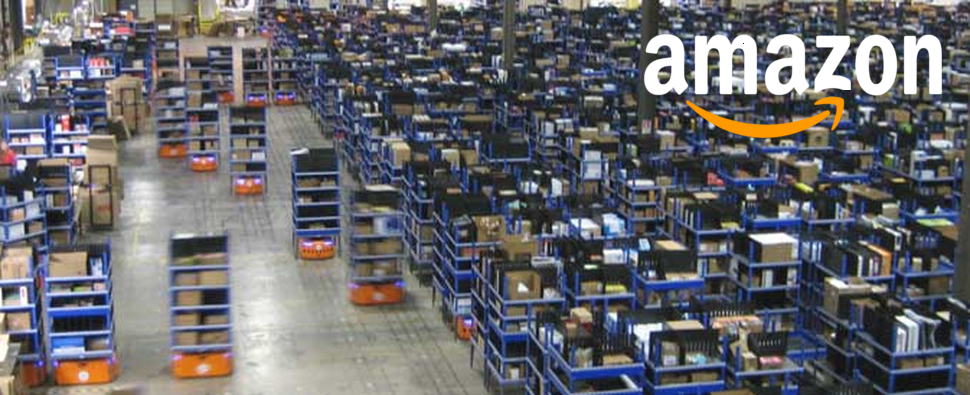
\includegraphics[width=\textwidth]{img/kiva.png}
        \end{figure}
        
        \begin{center}
        Kiva warehouse-management system
        \end{center}
    \end{frame}

    \begin{frame}[fragile]{Thesis contribution}
        \begin{center}
        The contribution of this thesis:
        \end{center}
        \begin{columns}
            \begin{column}{.7\textwidth}
           
            \begin{itemize}
            \item extension of  \texttt{ROS}  package
            \item proposing three tequnique:
            \begin{enumerate}
                \item Single robot : Single task (SR:ST) 
                \item Set Partition Strategy - Single robot : Multiple task (SPS1:N)
                \item Greedy Set Partition Strategy - Single robot : Multiple task (GSP1:N)
            \end{enumerate}
                \item real scenario: Computer Engineering for Industry 4.0 Laboratory (ICE Lab) 
            \end{itemize}
            \end{column}
            \begin{column}{.4\textwidth}
            \begin{figure}
                \subfloat{
\includegraphics[scale=0.45]{img/ros}}\qquad
                \subfloat{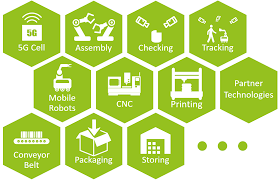
\includegraphics[scale=0.45]{img/ice}}
            \end{figure}
            \end{column}
        \end{columns}
    \end{frame}


    \begin{frame}[fragile]{ICE Laboratory}
        \begin{figure}[hbt]
            \centering
            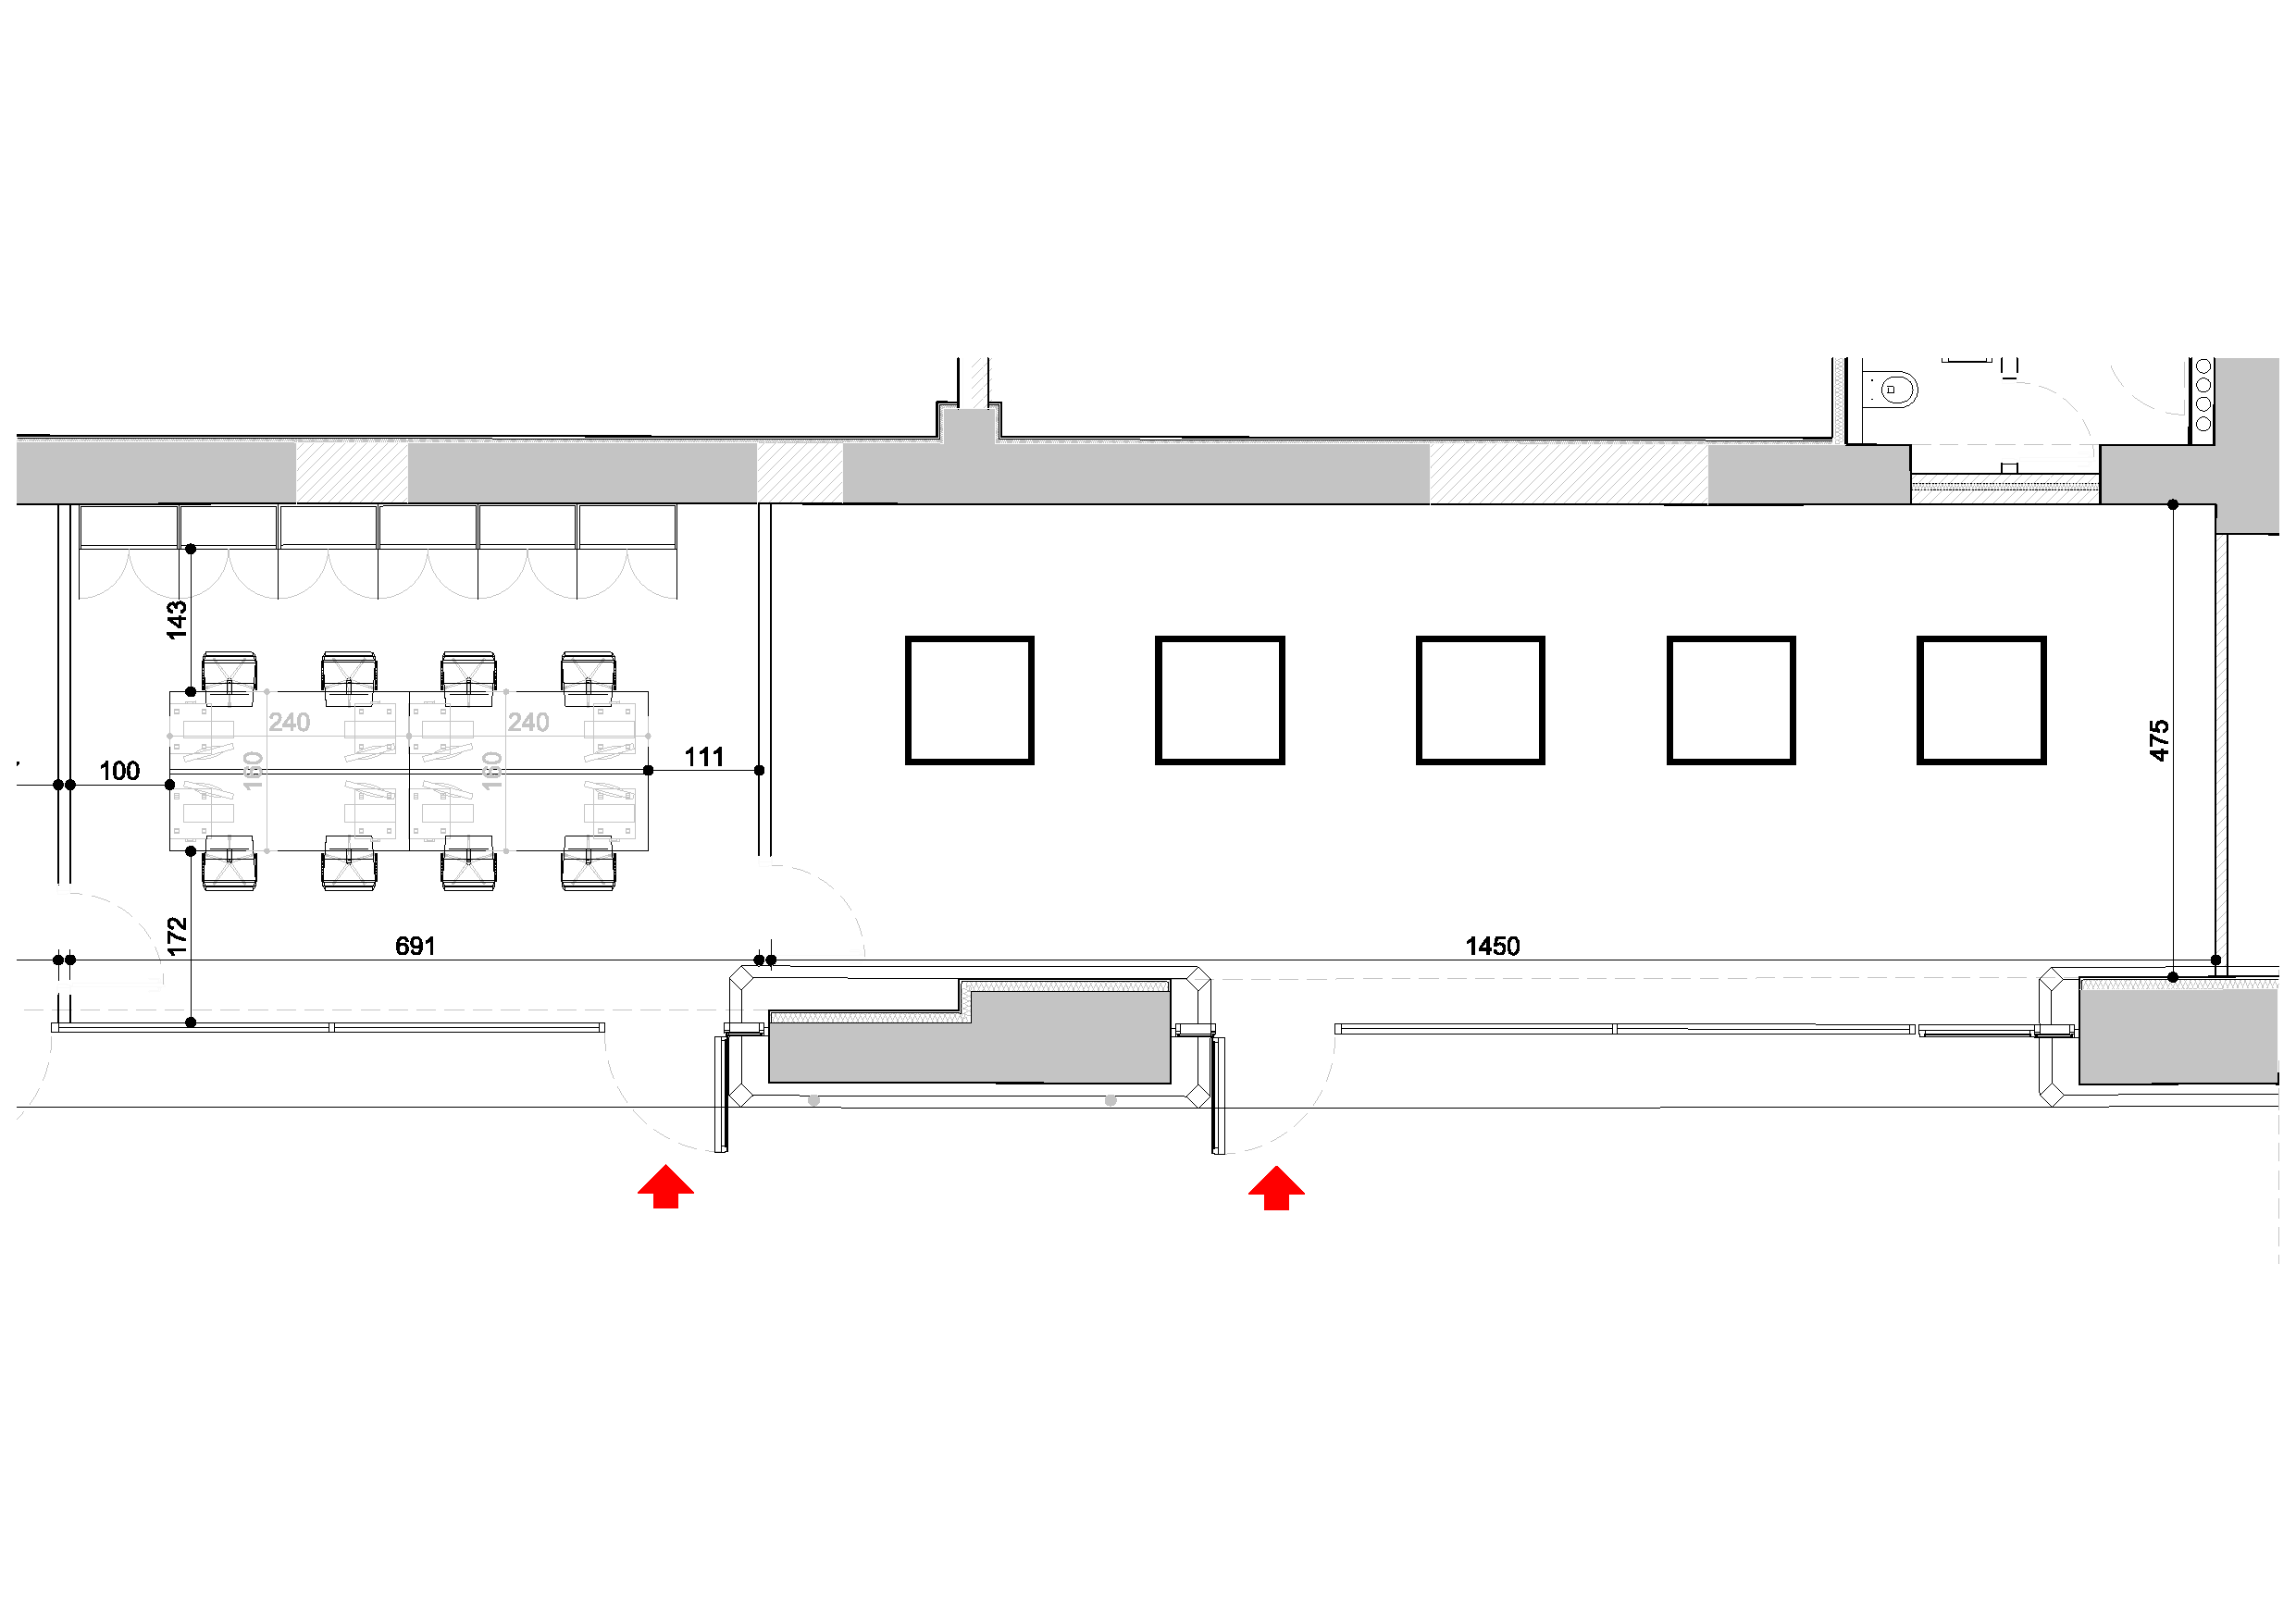
\includegraphics[width=\textwidth]{img/model1}
        \end{figure}
    \end{frame}

    \begin{frame}[fragile]{ICE Laboratory for logistic application}
        \begin{figure}[hbt]
            \centering
            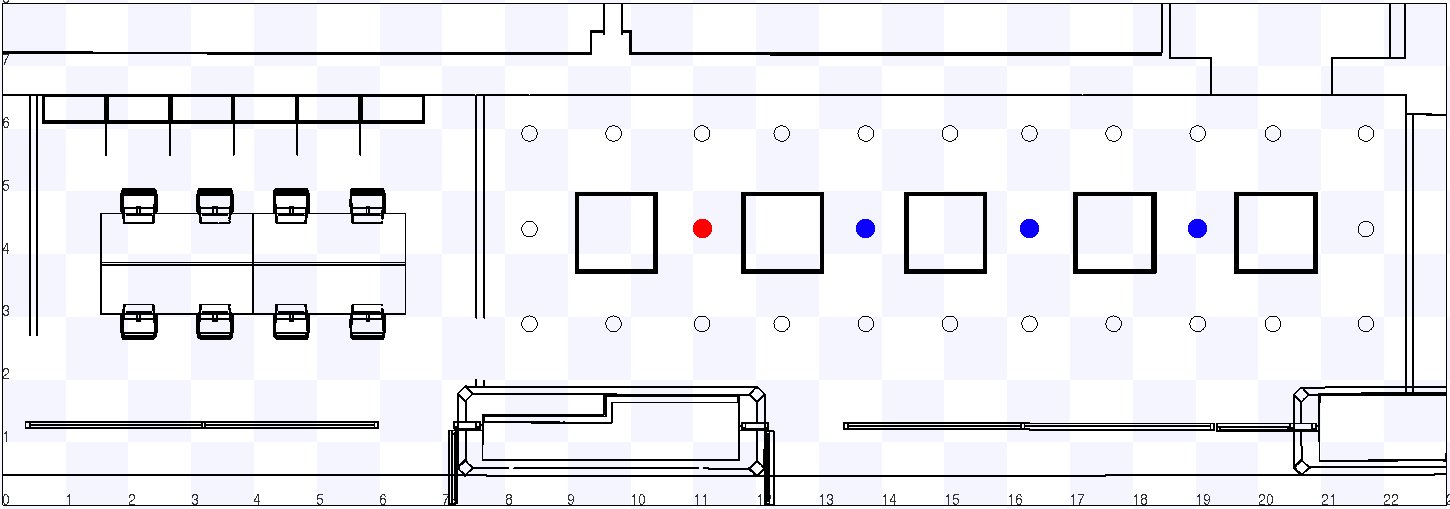
\includegraphics[width=\textwidth]{img/labgrafo}
        \end{figure}

        {\color{red}{$\bullet$}}  Loading bay
        \\
        {\color{blue}{$\bullet$}}  Unloading bays
        \\
        {\color{black}{$\circ$}}  Vertices
    \end{frame}

    \begin{frame}[fragile]{Set Partition Strategy - Single robot : Multiple task (SPS1:N)}
         \begin{columns}
            \begin{column}{.7\textwidth}
                \begin{center}
                    \begin{tabular}{|c|r|c|} \hline
                    \textbf{iteration} & \textbf{partition size} & \textbf{partition} \\ \hline
                    1    & 1    & \{\{a, b, c, d\}\}   \\
                    2    & 2    & \{\{a, b, c\}, \{d\}\}   \\
                    3    & 2    & \{\{a, b, d\}, \{c\}\}   \\
                    4    & 2    & \{\{a, b\}, \{c, d\}\}   \\
                    5    & 3    & \{\{a, b\}, \{c\}, \{d\}\}   \\
                    6    & 2    & \{\{a, c, d\}, \{b\}\}   \\
                    7    & 2    & \{\{a, c\}, \{b, d\}\}   \\
                    8    & 3    & \{\{a, c\}, \{b\},\{d\}\}   \\
                    9    & 2    & \{\{a, d\}, \{b, c\}\}   \\
                    10   & 2    & \{\{a\}, \{b, c, d\}\}   \\
                    11   & 3    & \{\{a\}, \{b, c\}, \{d\}\}   \\
                    12   & 3    & \{\{a, d\}, \{b\}, \{c\}\}   \\
                    13   & 3    & \{\{a\}, \{b, d\}, \{c\}\}   \\
                    14   & 3    & \{\{a\}, \{b\}, \{c, d\}\}   \\
                    15   & 4    & \{\{a\}, \{b\}, \{c\},\{d\}\}   \\ \hline       
                    \end{tabular}
                  \end{center}
            \end{column}
            \begin{column}{.4\textwidth}
            \begin{figure}
                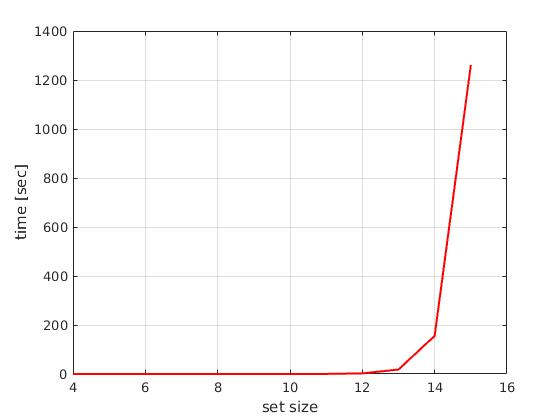
\includegraphics[width=\textwidth]{img/exp}
            \end{figure}
            \end{column}
        \end{columns}
    \end{frame}

    \begin{frame}[fragile]{Greedy Set Partition Strategy - Single robot : Multiple task (GSP1:N)}
    \end{frame}

    \begin{frame}[fragile]{ROS package Logistic\_sim}
        \begin{figure}[hbt]
            \centering
            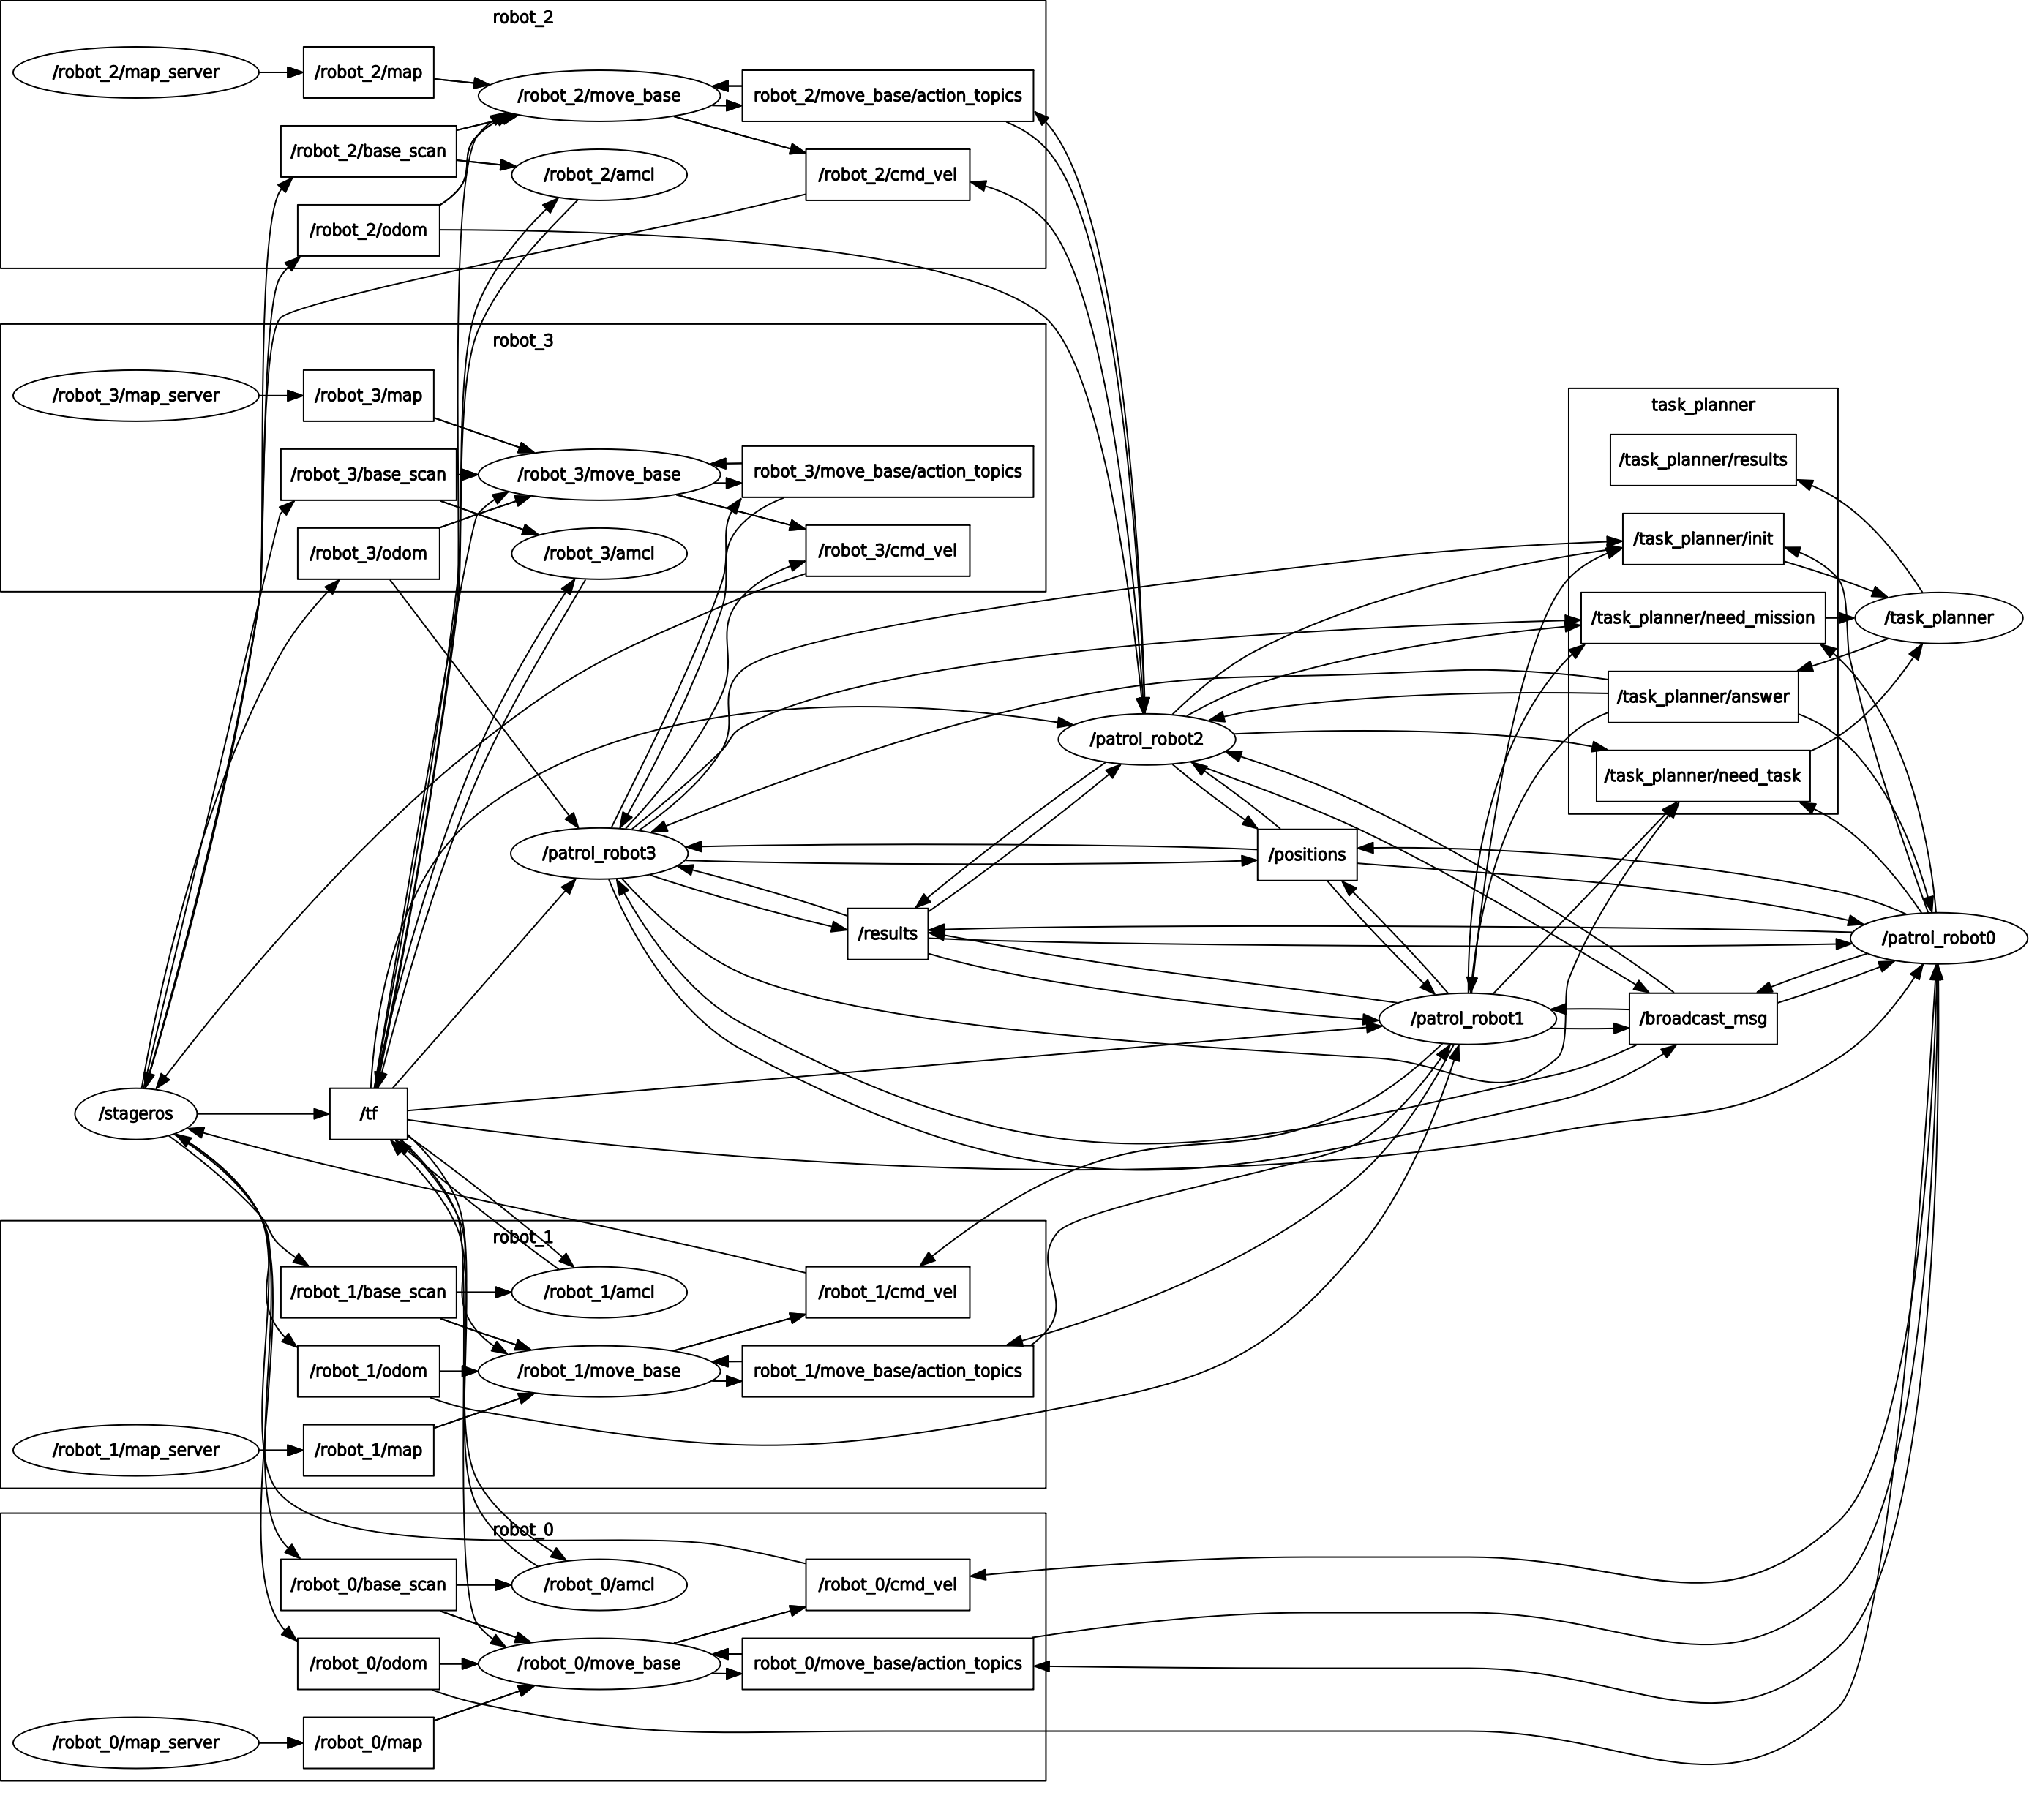
\includegraphics[scale=0.12]{img/rosgraph}
        \end{figure}
    \end{frame}

    \begin{frame}[fragile]{Empirical Results}
    \end{frame}

    \begin{frame}[fragile]{Video}
    \end{frame}

    \begin{frame}[fragile]{Conclusions and Future Work}
    \end{frame}









\chapter{Background and Related Works}\label{chap:related}
In this section, we detail the main issues for \mrs coordination 
in industrial domains, then we provide a detailed discussion on coordination
approaches, highlighting challenges and main solution techniques.

\section{Multi-Robot System for Industrial Applications}
In this thesis we also focus on industrial scenarios where robots have a high
degree of autonomy and operate in a dynamic environment.
\\
In article \cite{maxsum} robots must cooperate to maximizes the number of packages
completed in the unit of time. To this end a crucial component is to avoid interferences
when moving in the enviroment. They have formalised that problem as a Distributed 
Constrained Optimization problem based their solution on the binary max-sum algorithm.
\\
The most recent paper in logistic scenario \cite{mapd}, uses a Token Passing approach 
that solves the pickup-and-delivery tasks. The resulting algorithm takes kinematic 
constraints during planning, computes continuos agent movements with given velocities
that work on non-holonomic robots.

In this work, we consider a similar setting where a set of robots are involved
in trasportations tasks for logistics. However, we focus on the specific problem
of task assignment.

\section{Coordination in Multi-Robot system}
Coordination for \mrs has been investigated from several diverse
perspectives and nowadays, there is a wide range of techniques that can be used to 
orchestrate the actions and movements of robots operationg in the same enviroment.
Specifically, the ability to effectively coordinate the actions of a \mrs is a key 
requirement in several applications domains that range from disaster response to 
environmental monitoring, militaty operations, manufacturing and logistics. 
In all such domains, coordination has been addressed using various frameworks and 
techniques and there are several survery papers dedicated to categorize such different
approaches and identifying most prominent issues when developing \mrs.
\\
In the paper \cite{cooros} present and evaluate new ROS package for coordinated 
multi-robot exploration. The packages allow completely distributed control and do 
not rely on (but allow) central controllers.
\\
Given our focus on logistic scenarios, here we restrict our attention to coordination
approaches based on optimization and specifically on task assignment as this the most 
common framework for my reference application domain.

\chapter{Multi-Robot task allocation for pick-up and delivery}\label{chap:problem}
In this section we detail our reference scenario for MRS coordination and as well 
as the formalization of the problem we addressed and the solutions we propose.

\section{Description}
Our reference scenario is based on a warehouse that stores items of various types.
Such items must be composed together to satisfy orders that arrive based on customers’ demand.
The items of various types are stored in particular sections of the building (\textit{loading bay})
and must be trasported to a set of \textit{unloading bays} where such items are then 
packed together by human operators. The set of items to be trasported and where they should
go depends on the orders.

In our domain a set of robots is responsible for transporting items from
the loading bays to the unloading bays and the system goal is to maximize the
throughput of the orders, i.e., to maximize the number of orders completed in
the unit of time. Now, robots involved in transportation tasks move around
the warehouse and are likely to interfere when they move in close proximity,
and this can become a major source of inefficiency (e.g., robots must slow down
and they might even collide causing serious delays in the system).

Hence, a crucial aspect to maintain highly efficient and safe operations is to minimize the
possible spatial interferences between robots.
%  dire che ci focaliziamo sull'unione di pezzi del path


\section{Fomalization}
In this section we formalize the MRS coordination problem described above as a task allocation problem
where the robots must be allocated to transportation tasks. 

In our formalization we have a finite set of task. A robot can execute a task if it is available else the robot will go at start position.
For how the system is built, a robot to request a task must arrive at the previous vertex of the loading bay.

In more detail, our model considers a set of items of different types $E = \{ e_1,...,e_N\}$,
stored in a specific loading bay ($L$). The warehouse must serve a set of orders 
$O=\{o_1,...,o_M\}$. Orders are processed in one or more than one of the unloading bays ($U_i$).
Each order is defined by a vector of demand for each item type (the number of required 
items to close the order). Hence, $o_j = < d_{1,j},...,d_{N,j}>$, where $d_{i,j}$ is the 
demand for order $j$ of items of type $i$. When an order is finished a new one arrives,
until the set of task is finished.
The orders induce a set of $N \times M$ trasportation tasks $T = {t_{i,j}}$, with 
$t_{i,j} = < d_{i,j}, dst_{i,j}, P_{i,j}>$, where $t_{i,j}$ defines the task of transporting 
$d_{i,j}$ items of type $i$ for order $o_j$ (hence to unloading bay $U_j$).
Each task has a destination bay for centralized coordination the $t_{i,j}$ has a set of edges
$P_{i,j}$ which respects the strategy used. 
We have a set of robot $R = \{r_1,...,r_K \}$ that can execute transportation tasks, where
each robot has a defined load capacity for each item type $C_k = <c_{1,k},...,c_{N,k}>$, 
hence $c_{i,k}$ is the load capacity of robot $k$ for items of type $i$.

We consider in our logistic scenario, homogenous robots, which have the same radius 
and the same capacity. Because often in the logistic environments robots are all 
equal. 



In this section I propose the approaches with centralized coordination.
The first strategy, mentioned above, is the CGS1:1 which consider only 
one task allocated for one robot.
The second strategy extends the first, the main concept of this strategy 
is merging the tasks for optimaze the capacity of robot.

\section{Greedy Strategy Single robot : Single task (GS1:1)}





\section{Set Partition Strategy Single robot : Multiple task (SPS1:N)}





\section{Coalition formation Strategy Single robot : Multiple task (CFS1:N)}



% \chapter{Solution}\label{chap:solution}

\chapter{Empirical Setting} \label{chap:ros}
Writing software for robots is difficult, particularly as the scale and scope
of robotics continues to grow. Different types of robots can have wildly varying
hardware, making code reuse non trivial. On top of this, the magnitude of
the required code can be daunting, as it must contain a deep stack starting
from driver-level software and continuing up through perception, abstract
reasoning, and beyond.

\section{Robot Operating System (ROS)}
Our choice fell on ROS (Robot Operating System) which is a widespread
open-source, meta-operating system for a robot. It provides several services
that are commonly offered by an operating system, including hardware
abstraction, low-level device control, implementation of commonly-used functionality,
message-passing between processes, and package management. It is
worth noting that the full source code of ROS is publicly available, ROS is
distributed under the terms of the BSD license, which allows the development
of both non-commercial and commercial projects.

\subsection{Nomencalture and Architecture}
In this section we simply outline the terminology adopted in the ROS
community to allow an easy comprehension of the following discussion.
\\
The fundamental concepts of the ROS implementation are \textit{nodes}, \textit{messages},
\textit{topics}, and \textit{services}.
In ROS a system is typically comprised of many nodes. In this context, the term
\textit{"node"} is interchangeable with \textit{"software module"}. The use of term 
\textit{"node"} arises from visualization of ROS-based systems at runtime:
when many nodes are running, it is convenient to render the peer-to-peer communications
as a graph, called the \textit{computation graph}, with process as graph nodes and 
the peer-to-peer links as arcs.
\\
Nodes communicate with each other by passing \textit{messages}. A message is a
a strictly typed data structure. Standard primitive types (integer, floating
point, boolean, etc.) are supported, as are arrays of primitive types and
constants. Messages can be composed of other messages, and arrays of other
messages, nested arbitrarily deep. Messages descriptions are usually stored
in \texttt{my\_package/msg/MyMessageType.msg} and define the data structures for
messages sent in ROS, called custom message.
\\ 
Here is a simple example of a \texttt{*.msg} file that uses a header, some integer primitive,
arrays of integer and array of other \texttt{*.msg} files. The message is specified 
in a language neutral interface definition language (IDL) which uses very short text 
files to describe its fields and allow an easy composition of complex messages:
\begin{multicols}{2}
\begin{lstlisting}
    Header      header
    bool        take
    bool        go_home
    uint32      ID_ROBOT
    uint32      item
    uint32      order
    uint32      demand
    uint32      dst
    uint32      path_distance
    uint32[]    route
\end{lstlisting}
The custom message above rappresent a \texttt{Task.msg} which contains the basic
information to define a task in the system. Instead, the custom message below, rappresent 
a \texttt{Mission.msg} which is composed of task messages addressed to a specific robot.  
\begin{lstlisting}
    Header      header
    uint32      ID_ROBOT
    uint32      capacity
    Task[]      Mission
\end{lstlisting}
\end{multicols}

These simple high-level message definitions is then parsed and processed by a code 
generator module, one for each support language (currentrly \texttt{C++}), which generates 
native implementations that “feel” like native objects, and are automatically 
serialized and deserialized by ROS as messages are sent and received.
\\
A node sends a message by publishing it to a given \textit{topic}, which is simply
a string such as \texttt{/topic} or \texttt{/pkg/topic}. A node that is interested
in a certain kind of data will subscribe to the appropriate topic. There may be multiple
concurrent publishers and subscribers for a single topic, and a single node
may publish and/or subscribe to multiple topics. In general, publishers and
subscribers are not aware of each other existence (decoupling). 
% Figure TODO: report an example \textit{computation graph}
It is important to point out that because nodes connect to each other at runtime,
the graph can be \textit{dynamically} modified.
\\
Although the topic-based publish-subscribe model is a flexible communications
paradigm, its “broadcast” routing scheme is not appropriate forsynchronous transactions,
which can simplify the design of some nodes.
For this purpose ROS includes the concept of \textit{services}, defined by a string name
and a pair of strictly typed messages: one for the request and one for the
response. A providing node offers a service under a name and a client uses
the service by sending the request message and awaiting the reply.
\\
As for the topic-based paradigm a high-level description of a service is then
parsed and processed by a code generator module which generates the corresponding
native implementation in a supported target language.
Usually \texttt{C++} messages are generated in \texttt{my\_package/msg\_gen/cpp/include/my\_package},
while \texttt{C++} services are generated in \texttt{my\_package/srv\_gen/cpp/include/my\_package}.
% TODO figura di differenze tra topic e service
To support collaborative development, the ROS software system is organized into \textit{packages}.
A ROS package is simply a directory which contains an XML file describing the package
and stating any dependencies. A collection of ROS packages is a directory tree with ROS
packages at the leaves: a ROS package repository may thus contain an arbitrarily complex
scheme of subdirectories. This structure is primarily meant to partition the building of 
ROS-based software into small, manageable chunks of functionality.
\\
In ROS, a \textit{stack} of software is a cluster of nodes that does something
coherent as a whole, as is illustrated in the simple \textit{navigation} example reported
in Figure. %TODO 
To allow for “packaged” functionality such as a navigation system, ROS provides
a tool called \texttt{roslaunch}, which reads an XML-like description of a graph and instantiates
the graph on the cluster, optionally on specific hosts.
Thus ROS is able to instantiate a set of nodes with a single
command, once the nodes are described in a \texttt{launch} file, the simple usage
is:
\begin{lstlisting}
    roslaunch [package] [filename.launch]
\end{lstlisting}

\subsection{The Stage 2D Simulation}
For visualization purposes we adopted the Stage 2D robot simulator
which provides a virtual world populated by mobile robots and enriched with
sensors, actuators and both approximate and exact localization. Stage is
designed to be sufficiently simple to allow an easy set-up but at the same time
it is intended to be just realistic enough to enable users to move controllers
directly between Stage robots and real robots. 
\\
Stage is made available in ROS with the \texttt{stageros} node which wraps the 
simulator and exposes its functionality to the rest of the system. The following 
code reports how it is launched:

\begin{lstlisting}
<?xml version="1.0" encoding="UTF-8" ?>
<launch>
    <arg name="map" default="grid" />
    <arg name="stage_pkg" default="stage_ros"/>     
    <arg name="custom_stage" default="false" />
    <group unless="$(arg custom_stage)"> 
        <node name="stageros" pkg="$(arg stage_pkg)" type="stageros" 
        args="$(find patrolling_sim)/maps/$(arg map)/$(arg map).world" 
        output="screen" />
    </group>
</launch>
\end{lstlisting}

The \texttt{*.world} file specified tells Stage everything about the world,
from obstacles (usually represented via a \texttt{*.pgm} image), to robots and other 
objects. In particular, after the definition of some parameters related to general 
camera and GUI options, we specify the static map on which the robot has to navigate 
(we will describe its characteristics shortly) and finally we include two specific 
files which aims defining the properties of respectively the laser sensor and the robot.
The last instruction just throws the robot in the map by indicating it's $x$, $y$, $z$
and $\theta$ coordinates, this is summarized in:
\begin{lstlisting}
include "../hokuyo.inc"
include "../crobot.inc"
include "../floorplan.inc"
include "../cpoint.inc"
window
( size   [ 460 180 1 ]         
  rotate [ 0.000 0.000 ]    
  center [ 11.5 4.0 ]   
  scale 20
  show_data 1)
floorplan
( size [23.0 8.0  1] 
  pose [11.5 4.0 0 0]
  bitmap "model5.pgm")
include "robots.inc"
include "point.inc"
\end{lstlisting}
The first included file (hokuyo.inc) defines the physical and technical
properties of the particular laser range finders support that we adopt: we
define it to have a circular shape and to be mounted on top of the robot base
which has the same circular shape. As for the sensor properties we specify
the following parameters described in:
\begin{lstlisting}
define hokuyo ranger
(sensor(           
    range [ 0.0  5.0 ] # the max/min range reported by the scanner, in meters.
    fov 230            # the angular field of view of the scanner, in degrees.
    samples 1081       # the number of laser samples per scan.)
  # model properties
  color "orange"
  size [ 0.1 0.1 0.1 ]
  block( points 4
    point[0] [0 0]
    point[1] [0 1]
    point[2] [1 1]
    point[3] [1 0]
    z [0 1]))
\end{lstlisting}
The second included file (crobot.inc) defines the physical properties of
the robot, as mentioned above we define it to have a circular shape which
is suffice for our purpose of having a mobile camera that moves around the world:
\begin{lstlisting}
    define crobot position(
    size [0.3 0.3 0.2]
    origin [0 0 0 0]
    gui_nose 0
    drive "diff"
    # This block approximates a circular shape of a Robot
    block( points 16
        point[0] [ 0.225 0.000 ]
        point[1] [ 0.208 0.086 ]
        point[2] [ 0.159 0.159 ]
        point[3] [ 0.086 0.208 ]
        point[4] [ 0.000 0.225 ]
        point[5] [ -0.086 0.208 ]
        point[6] [ -0.159 0.159 ]
        point[7] [ -0.208 0.086 ]
        point[8] [ -0.225 0.000 ]
        point[9] [ -0.208 -0.086 ]
        point[10] [ -0.159 -0.159 ]
        point[11] [ -0.086 -0.208 ]
        point[12] [ -0.000 -0.225 ]
        point[13] [ 0.086 -0.208 ]
        point[14] [ 0.159 -0.159 ]
        point[15] [ 0.208 -0.086 ]
        z [0 1])
    hokuyo( pose [0.15 0 -0.1 0] )
    # Report error-free position in world coordinates
    localization "gps"
    #localization_origin [ 0 0 0 0 ]
    # Some more realistic localization error
    localization "odom"
    odom_error [ 0.01 0.01 0.0 0.1 ])
\end{lstlisting}
% TODO sistemare gli spazzi bianchi

\section{Localization and Navigation}
Purpose of this section is to describing how we address the two main problems in
the context of mobile robotics: \textit{localization} and \textit{navigation}.
The former deals with tracking the pose of the robot during its motion allowing
it to localize itself in the map, the latter deals with driving the robot from a 
starting position to a goal position trying to avoid potential obstacles.

{\bf TODO: Figura della simulazione}
\newpage
\subsection{Mapping}
The robot navigation system can be initialized with or without an a priori, \textit{static map}.
When initialized without a map, the robot only knows about obstacles that it has seen,
and will make optimistic global plans through areas that it has not yet visitied
which may traverse unknown space, potentially intersecting unseen obstacles. 
As the robot receives more information about the world, it replans accordingly to
avoid obstacles. Initialized with a static map, the robot will make informed plans 
about distant parts of the environment, using the map as prior obstacle information.
In our case we provide ROS with a static map of real laboratory in University of Verona.
Doing so requires us to set the \textit{map\_server} node that reads a map from 
disk and offers it via a ROS service:
\begin{lstlisting}
<!-- Run the map server -->
<node name="map_server" pkg="map_server" type="map_server" 
args="$(find patrolling_sim)/maps/$(arg mapname)/$(arg mapname).yaml" />
\end{lstlisting}
The current implementation of \textit{map\_server} convert color values in the map 
image data into ternary occupancy values: \textit{free}(0), \textit{occupied}(100), and
\textit{unknown}(-1).
\\
Maps manipulated by the tools in the \textit{map\_server} package are stored in a 
pair of file: the \texttt{*.yaml} file describes the map meta-data and names the image 
file while the image file encodes the occupancy data.
\\
The \texttt{*.yaml} file given as an argument to the \textit{map\_server} node is reported
below with a brief description of it's parameters.
\begin{lstlisting}
# path to the image file containing the occupancy data.
image: src/patrolling_sim/maps/model5/model5.pgm
# resolution of the map, meters/pixel.
resolution: 0.014100
# the 2-D pose of the lower-left pixel in the map, as (x, y, yaw).
origin: [0.000000, 0.000000, 0.000000]
# whether the white/black free/occupied semantics should be reversed.
negate: 0
# pixels with occupancy probability greater than 
# this are considered completely occupied.
occupied_thresh: 0.65
# pixels with occupancy probability less than 
# this are considered completely free.
free_thresh: 0.196
\end{lstlisting}

\subsection{Localization}
Both in the case of a given static map or without a given static map, we
require that the robot’s pose be tracked in a consistent global coordinate frame.
When not using a map, the robot’s pose is usually estimated by integrating
wheel odometry, possibly fused with data from an inertial measurement unit
(IMU). When using a map, as in our case, the robot is usually localized using
a probabilistic technique, in particular we adopt the Adaptive Monte Carlo
Localization (\texttt{amcl}) system:
\begin{lstlisting}
<group if="$(arg use_amcl)">
    <!--- AMCL -->
    <include file="$(find patrolling_sim)/params/amcl/amcl_diff.launch" />       
    <!-- Override AMCL Frame Params to include prefix -->
    <param name="/$(arg robotname)/amcl/base_frame_id" 
        value="$(arg robotname)/base_link"/>
    <param name="/$(arg robotname)/amcl/odom_frame_id" 
        value="$(arg robotname)/odom"/>
    <!--common map frame for all robots -->
    <param name="/$(arg robotname)/amcl/global_frame_id" value="map"/> 
</group>
\end{lstlisting}
\texttt{amcl} is a probabilistic localization system for a robot moving in 2D.
It implements the Adaptive (or KLD-sampling) Monte Carlo Localization
approach which uses a particle filter to track the pose of a robot against
a known map. The map of the environment where the robot has to localize
itself must be given to the robot beforehand. In our case the map is provided
by tha \textit{map\_server} node. This map is the so called \textit{occupacy map}
like before mentioned: it contains a value for every location which indicates the 
probability that this location is occupied by an object such as a wall. 
\texttt{amcl} takes in a laser-based map, laser scans and outputs pose estimates.
On startup, \texttt{amcl} initializes its particle filter according to the parameters
provided. In this respect we remark that the \texttt{amcl} node is launched only 
after having setting up three categories of ROS parameters that we use to configure 
its behaviour: \textit{overall filter}, \textit{laser model} and \textit{odometry model}.
The complete configuration file is reported below.
\begin{lstlisting}
<?xml version="1.0" encoding="UTF-8" ?>
<launch>
<arg name="robotname" default="robot_0" />
<node pkg="amcl" type="amcl" name="amcl" args="scan:=base_scan">
  <!-- Publish scans from best pose at a max of 10 Hz -->
  <param name="odom_model_type" value="diff"/>
  <param name="odom_alpha5" value="0.1"/>
  <param name="transform_tolerance" value="0.2" />
  <param name="gui_publish_rate" value="-10.0"/>
  <param name="laser_max_beams" value="30"/>
  <param name="min_particles" value="100"/>
  <param name="max_particles" value="500"/>
  <param name="kld_err" value="0.05"/>
  <param name="kld_z" value="0.99"/>
  <param name="odom_alpha1" value="0.2"/>
  <param name="odom_alpha2" value="0.2"/>
  <!-- translation std dev, m -->
  <param name="odom_alpha3" value="0.8"/>
  <param name="odom_alpha4" value="0.2"/>
  <param name="laser_z_hit" value="0.5"/>
  <param name="laser_z_short" value="0.05"/>
  <param name="laser_z_max" value="0.05"/>
  <param name="laser_z_rand" value="0.5"/>
  <param name="laser_sigma_hit" value="0.2"/>
  <param name="laser_lambda_short" value="0.1"/>
  <param name="laser_lambda_short" value="0.1"/>
  <param name="laser_model_type" value="likelihood_field"/>
  <!-- <param name="laser_model_type" value="beam"/> -->
  <param name="laser_likelihood_max_dist" value="2.0"/>
  <param name="update_min_d" value="0.2"/>
  <param name="update_min_a" value="0.5"/>
  <param name="odom_frame_id" value="odom"/>
  <param name="base_frame_id" value="base_link"/>
  <param name="resample_interval" value="1"/>
</node>
</launch>
\end{lstlisting}

\subsection{Navigation}
At high level the navigation system is quite simple. It takes in data from sensors,
odometry, and a navigation goal, and outputs velocity commands that are sent to a 
mobile base. The low-level architecture of system, however, is complex and consist 
of many components that interacts together.
\\
For navigation purposes we rely on the \textit{move\_base} package which provides 
an interface with the entire ROS navigation stack. The \textit{move\_base} package
provides an implementation of an \textit{action} that, given a goal in the world,
will attempt to reach it with a mobile base. It links together a \textit{global} and 
\textit{local} planner to accomplish its navigation task, it also maintains two 
costmaps, one for the global planner and one for the local planner.
An architecture view of the node its interaction with other components is show in 
Figure below. %TODO

The pre-requisites of navigation stack, along with a brief description of it's main 
components, are provided in the section below.
\subsection*{Trasformations}
Robotics systems often need to track spartial relationships between \textit{frames}
for a variety of reasons: between a mobile robot and some fixed frame of reference 
for localizzation or, as in our case, between the frame related to the mobile base 
and the one related to the laser sensor. To simplify the treatment of spartial frames,
a trasformation system has been written for ROS, called \texttt{tf}. The \texttt{tf} system 
constructs a dynamic \textit{trasformation tree} which realtes all frames of reference 
in the system. At an abstract level, a trasformation tree define \textit{offsets}
in terms of both translation and rotation between different coordinate frames.
\\
Referring to our case of a simple robot consisting of a circular mobile base
with a single laser support mounted on top of it we define two coordinate
frames: one corresponding to the center point of the base of the robot and one
for the center point of the laser support that is mounted on top of the base.
We've called the coordinate frame attached to the modile base \texttt{base\_link}
and the coordinate frame attached to the laser support \texttt{base\_laser\_link}.
Once this configuration in defined, every time that we have some data from the laser 
in the form of distances from the laser's center point and we want to take this data 
and use it to help the mobile base avoid obastacles in the world we invoke the \texttt{tf}
system which in the general case transforms the information towards the \texttt{base\_link}
coordiante frame. Below we reported the Figure which rappresent the configuration of 
\texttt{base\_link} and the \texttt{base\_laser\_link} frames.
%TODO figure of robot.
Our robot can thus use this information to reason about laser scans in
the \texttt{base\_link} frame and safely plan around obstacles in its environment.

\subsection*{Sensor Information}
The navigation stack uses information from sensors to avoid obstacles in the world,
it assumes that these sensors are publishing either \texttt{sensor\_msgs/LaserScan}
or \texttt{sensor\_msgs/PointCloud} message over ROS.
Publishing data correctly from sensors over ROS is important for the
navigation stack to operate safely. If the navigation stack receives no information
from a robot’s sensors, then of course it will drive blindly and, most
likely, hit things.
%TODO figure of one robot on map with laser 
Our \texttt{sensor\_msgs/LaserScan} message type, like many other messages sent 
over ROS, contain \texttt{tf} frame and time dependent information. To standardize 
how this information is sent, the \texttt{Header} message type is used as field
in all such messages.
The three field in the \texttt{Header} type are show below.
 %inserti image Header message laser scan
\begin{lstlisting}
# Standard metadata for higher-level flow data types
uint32 seq
time stamp
string frame_id
\end{lstlisting}
The \texttt{seq} field corresponds to an identifier that automatically increases
as messages are sent from a given publisher. The \texttt{stamp} field stores time 
information that should be associated with data in a message. The \texttt{frame\_id}
field stores \texttt{tf} frame information that should be associated with data 
in a message. 
The body of the \texttt{sensor\_msgs/LaserScan} message holds informations about 
any given scan and contains the associated geometric informations in the following
form:
\begin{lstlisting}
# Laser scans angles are measured counter clockwise, with 0 facing forward
Header header
float32 angle_min # start angle of the scan [rad]
float32 angle_max # end angle of the scan [rad]
float32 angle_increment # angular distance between measurements [rad]
float32 time_increment # time between measurements [seconds]
float32 scan_time # time between scans [seconds]
float32 range_min # minimum range value [m]
float32 range_max # maximum range value [m]
float32[] ranges # range data [m] (Note: values < range_min or > range_max
should be discarded)
float32[] intensities # intensity data [device-specific units]
\end{lstlisting}

\subsection*{Odometry Informations}
The navigation stack requires that odometry information be published using 
\texttt{tf} and the \texttt{nav\_msgs/Odometry} message. The last message in 
required because \texttt{tf} alone does not provide any information about the 
velocity of the robot, it is thus required that any \textit{odometry source} 
publishes both this kind of information to \textit{move\_base}.
\\
The \texttt{nav\_msgs/Odometry} message stores an estimate of the position and 
velocity of a robot in free space:
\begin{lstlisting}
# The pose in this message should be specified in the coordinate frame given
by header.frame_id.
# The twist in this message should be specified in the coordinate frame
given by the child_frame_id
Header header
string child_frame_id
geometry_msgs/PoseWithCovariance pose
geometry_msgs/TwistWithCovariance twist
\end{lstlisting}
The \textit{pose} in this message corresponds to the estimated position of the 
robot in the odometric frame of reference along with an optional covariance for 
the certainty of that pose estimate. The \textit{twist} in this message corresponds
to the robot's velocity in the child frame, normally the coordinate frame of the 
mobile base, along with an optional covariance for certainty of that velocity estimate.
\\
In our case since the \texttt{stageros} node represents the odometric source for 
the system,it is going to publish all the relevant trasformations between the
coordinate frames it manages towards the \texttt{/tf} topic which maintains the current 
trasformation tree for our system, and a \texttt{nav\_msgs/Odometry} message to 
the \texttt{/odom} topic so that the navigation stack can retrieve velocity information
from it.
%Image tf connection

\subsection*{Base Controller}
As previously specified the navigation stack assumes that it can send velocity commands
using a \texttt{geometry\_msgs/Twist} message assumed to be in the base coordinate
frame of the robot on the \texttt{/cmd\_vel} topic. This means there must be a node 
subscribing to the \texttt{/cmd\_vel} topic that is capable of talking 
$(v_x,v_y,v_\theta) \longleftrightarrow $ (\texttt{cmd\_vel.linear.x}, \texttt{cmd\_vel.linear.y}, \texttt{cmd\_vel.angular.z})
veloccities and converting them into motor commands to send a mobile base.
\\
In this work the \texttt{stageros} node subscribes to the \texttt{/cmd\_vel} topic
simulating the movement of a real robot in a real environment.

\subsection{Global and Local planner algorithms}
The \texttt{base\_local\_planner} is responsible for computing velicty commands
to send to the mobile base of the robot given a high-level plan. In particular,
this package adheres to the \texttt{BaseLocalPlanner} interface specified in the 
\texttt{nav\_core} package which provides common interfaces for both \textit{global}
and \textit{local} action planning.
\\
As we shall see, the local planner is seeded with the high-level plan produced by
the global planner and the purpose of the \texttt{nav\_core} package is just to 
provide common interfaces for navigation. 
\subsection*{Global planner}
The global planner is given the obstacle and cost information contained
in the global costmap, information from the robot’s localization system, and
a goal in the world. From these, it creates a high-level plan for the robot
to follow to reach the goal location. In more detail, the global planner will
create a series of way-points for the local planner to achieve, these way-points
assumes that the robot is circular in shape, and may in fact be infeasible for a
more general case. Also, the global planner doesn’t take the dynamics of the
robot into account so it can produce plans that are dynamically infeasible as
well. While this ensures that the global planner returns in a small amount of
time, it also means that the planner is \textit{optimistic} in the plans that it creates.
However our robot is not much affected by this problems because it is circular
in shape and does not have a particular dynamics to take into account.
\\
The global planner used for this nagivation system is \texttt{ROS navigation} stack
% wiki/ros/navigation / amcl
This planner, as started before, assumes a circular robot and operates on a costmap 
to compute a navigation function that can later be used to find a \textit{minimum cost plan}
from a start point to an end point in a grind.
\\
As outlined before, the global planner may produce a path for the robot that is infeasible,
such as a plan that turns through a narrow way too tightly, causing the corners of the 
robot to hit the surrounding obstacles. Because of its shortcomings, the global planner 
is used only as a high-level guide for navigation in an environment and we also need a 
\textit{local planner} for navigation.

\subsection*{Local planner}
The local planner is responsible for generating velocity commands for
the mobile base that will safely move the robot towards a goal. The local
planner is seeded with the plan produced by the global planner, and attempts
to follow it as closely as possible while taking into account the kinematics
and dynamics of the robot as well as the obstacle information stored in the
costmap.
\\
The local planner used for this navigation system is \texttt{base\_local\_planner}.
This package supports any robot footprint that can be represented as a convex
polygon or circle, so it is fine for our circular-shaped robot.
The \texttt{base\_local\_planner} package provides a \textit{controller} that drives
a mobile base in the plane. This controller serves to connect the path planner
to the robot. Using a map, the planner creates a trajectory for the robot to
move from a start to a goal location. Along the way, the planner creates, at
least locally around the robot, a value function, represented as a grid map.
This value function encodes the costs of traversing through the grid cells
based on their occupancy status. The controller uses this value function to determine 
$v_x$, $v_y$ and $v_\theta$ velocities to send to the robot.
\\
In order to generate safe velocity commands to send to the mobile base,
the local planner we adopt makes use of a technique known as the \textit{Dynamic
Window Approach} (DWA) to forward simulate and select among potential
commands based on a cost function. The basic idea is as follows:
\begin{itemize}
    \item First it discretely samples the robot’s control space (which means
    samples from the set of achievable velocities $v_x$, $v_y$ and $v_\theta$ for just one
    simulation step given the acceleration limits of the robot);
    \item Then for each sampled velocity, it performs forward simulation from
    the robot’s current state to predict what would happen if the sampled
    velocity were applied for some (short) period of time;
    \item Next it evaluates (score) each trajectory resulting from the forward
    simulation, using a metric that incorporates characteristics such as
    \textit{proximity to obstacles, proximity to the goal, proximity to the path produced 
    by the global planner and speed} and it discards illegal trajectories
    (those that collide with obstacles);
    \item Finally it picks the highest-scoring trajectory and sends the associated
    velocity to the mobile base;
    \item Rinse and repeat.
\end{itemize}
In order to score trajectories efficiently, a map grid is used. For each
control cycle, a grid is created around the robot (the size of the local costmap),
and the global path is mapped onto this area. This means some of the grid
cells will be marked with distance 0 to a path point, and distance 0 to the
goal. A propagation algorithm then efficiently marks all other cells with their
\textit{Manhattan distance} to the closest of the points marked with zero. The goal
of the global path may often lie outside the small area covered by the map
grid, so when scoring trajectories for proximity to goal, what is considered is
the “local goal”, meaning the first path point which is inside the area having
a consecutive point on the global path outside the area.
\\
We report here our configuration file for the local planner we adopt, it is
worth noting that through setting the weights on each component of the cost
function differently it is possible to change drastically the behaviour of the
robot: for example it is possible to force it to stay close to the projection of
the global path into the local costmap, or to stay quite far from obstacles
changing consequently it’s trajectory across the map. The values below works
well for our case since they take into account both the shape of the robot
and the needs for computation. For a detailed description parameters see code below.
\begin{lstlisting}
controller_frequency: 5.0
TrajectoryPlannerROS:
# Robot Configuration Parameters
max_vel_x: 1.00
min_vel_x: 0.10
max_trans_vel: 1.00
min_trans_vel: 0.10
max_rot_vel: 1.0
min_in_place_rotational_vel: 0.1
acc_lim_th: 0.75
acc_lim_x: 0.50
acc_lim_y: 0.50
holonomic_robot: false
# Goal Tolerance Parameters
yaw_goal_tolerance: 6.28
xy_goal_tolerance: 0.40
# Controller Parameters 
pdist_scale: 0.6
gdist_scale: 0.8
occdist_scale: 0.01 
meter_scoring: true
# Forward Simulation Parameters
sim_time: 1.5
vx_samples: 6
vtheta_samples: 20
# Trajectory Scoring Parameters
heading_lookahead: 0.325
dwa: true
# Oscillation Prevention Parameters
oscillation_reset_dist: 0.05
\end{lstlisting}

\section{Cost-maps configurations}
The navigation stack uses two costmaps to store information about obstacles in the world.
One costmap is used for \textit{global planning}, meaning creating long-term plans 
over the entire environment, and the other is used for \textit{local planning} and 
obstacle avoidance.
\\
In particular, the ROS package \texttt{costmap\_2D} provides an implementation
of a 2D costmap that takes in sensor data from the world, build a 2D occupacy 
grid of the data and inflates costs in a 2D costmap based on the occupacy grid 
and a user specified \textit{inflation radius}.
\\
Because the robots we study are constrained to drive on flat ground, and
cannot, for example, step or jump over obstructions, we assemble obstacle
data into a planar costmap on which the planners operates. The costmap is
initialized with our laboratory static map, but updates as new sensor data comes in
to maintain an up-to-date view of the robot’s local and global environment.
\\
As previously specified, the laboratory image describes the occupacy state of each 
cell of the map in the color of the corresponding pixel. Cells with occupacy 
probability greater than the value stored in \texttt{occuped\_thresh} are considered
completely occupied and are assigned a lethal cost, meaning that no part of the 
robot's circular footprint is allowed to be inside of the corresponding two-dimensional cell.
Then, inflation is performed in two dimension to propagate costs from obstacles out 
to user-specified \textit{inflation radius}. Cells that are less than one inscribed
radius of the robot away from an obstacle are assigned a uniformly high cost, after 
which an exponential decay function is applied that will cause the cost to decrease 
with the distance from the obstacles.

\subsection{Common configuration}
There are some configuration options that we want both global and local costmap 
to follow. In our case the global configuration settings for both the costmaps are 
as follows:
\begin{lstlisting}
obstacle_range: 0.50
raytrace_range: 3.0
robot_radius: 0.33
inflation_radius: 0.33
observation_sources: laser_scan_sensor
laser_scan_sensor: {sensor_frame: base_laser_link,
 data_type: LaserScan, topic: base_scan, marking: true, clearing: true}
\end{lstlisting}
The first two parameters set thresholds on obstacle information put into the 
costmap. The \texttt{obstacle\_range} parameters determines the maximum range sensor
reading that will result in an obstacle being put into the costmap.
The \texttt{raytrace\_range} parameter determines the range to which we will ray-trace 
freespace given a sensor reading.
\\
Next we set the radius of the robot since it is circular and the inflation radius 
for the costmap. The inflation radius should be set to the maximum distance 
from obstacles at which a cost should be incurred. 
\\
The \texttt{observation\_sources} parameter defines the sensor that is going to be passing 
information to the costmap, the last line sets it's parameters. The \texttt{sensor\_frame}
parameter is set to the name of the coordiante frame of the sensor, the \texttt{data\_type}
parameter is set to \texttt{LaserScan} since this is the type of message used by the topic,
and the \texttt{topic} parameter is set to the name of the topic that the sensor 
publishes data on. The \texttt{marking} and \texttt{clearing} parameters determine 
whether the sensor will be used to add obstacle information to the costmap, clear obstacle
information from the costmap, or do both.

\subsection{Global configuration}
Below are our configuration settings for the \textit{global} costmap along with a
description of their semantics:
\begin{lstlisting}
global_costmap:
   global_frame: /map
   robot_base_frame: base_link
   update_frequency: 3.0
   publish_frequency: 0.0
   static_map: true
   inflation_radius: 0.66
\end{lstlisting}

The \texttt{global\_frame} parameter defines what coordinate frame the costmap should
run in, in this case, we'll choose the \texttt{map} frame. The \texttt{robot\_base\_frame}
parameter defines the coordiante frame the costmap should reference for the base 
of the robot. The \texttt{update\_frequency} parameter determines the frequency, in Hz, 
at which the costmap will run its update loop. The \texttt{static\_map} parameter 
determines whether or not the costmap should initialize itself based on a map served 
by the \textit{map\_server}.

\subsection{Local configuration}
Below are our configuration settings for the \textit{local} costmap along with a 
description of their semantics:
\begin{lstlisting}
local_costmap:
   global_frame: odom
   robot_base_frame: base_link
   update_frequency: 3.0
   publish_frequency: 2.0
   static_map: false
   rolling_window: true
   width: 4.0
   height: 4.0
   resolution: 0.05
\end{lstlisting}
The \texttt{global\_frame}, \texttt{robot\_base\_frame}, \texttt{update\_frequency}
and \texttt{static\_map} parameters are the same as described previously.
The \texttt{publish\_frequency} parameter determines the rate, in Hz, at which 
the costmap will publish visualization information. Setting the \texttt{rolling\_window}
parameter to true means that the costmap will remain centered around the robot moves 
through the world. The \texttt{width}, \texttt{height} and \texttt{resolution} 
parameters set the width [m], height [m] and resolution [m/cell] of the costmap.

\subsection{Local and global coordinate frames}
We now briefly discuss why it is important to distinguish between global
and local coordinate frames when building a navigation system. A global
coordinate frame, such as the one used by the \textit{global planner} and specified
through the \texttt{global\_frame: /map} parameter, is advantageous in that it
provides a globally consistent frame of reference, but it is flawed in that it is
subject to discontinuous jumps in its estimation of the robot’s position. For
example, when the localization system is struggling to determine the robot’s
position, it is not uncommon for the robot to teleport, on a single update
step, from one location to another that is one meter away.
\\
A local coordinate frame, such as the one used by the \textit{local planner} and
specified through the \texttt{global\_frame: /odom parameter}, has no such jumps,
but presents its own flaws in that it is prone to drifting over time.
\\
In theory, all planning and obstacle avoidance could be performed in
the global frame, but this may lead to problems when discrete jumps in
localization occur. To illustrate this, consider the case in which a robot
navigates through a narrow way with limited clearance on either side. If the
navigation system attempts to plan in a global frame, localization jumps
may drastically affects the robot’s obstacle information and a jump in the
robot’s position of just a few centimetres to either side, combined with new
sensor data, may actually be enough for the robot to consider that way as
unfeasible. If the robot instead operates in a local frame, nearby obstacles
are not affected by jumps in localization, and the robot can traverse through
the way independently of any difficulties with the localization system.
Thus, we use the global coordinate frame to create high-level plans for
the robot but also a local coordinate frame for local planning and obstacle
avoidance. To relate the two frames, the plan produced by the global planner
is mapped from the global coordinate frame into the local coordinate frame
on every cycle.

\section{Recovery behaviours}
The navigation system as described until now works well most of the time,
attempting to achieve a goal pose with its base to within a user-specified
tolerance, but there are still situations where the robot can get stuck.
One common cause of failure for the navigation system is \textit{entrapment},
where the robot is surrounded by obstacles and cannot find a valid plan to its goal.
When the robot finds itself in this situation, a number of increasingly
aggressive recovery behaviours are executed to attempt to clear out space,
Figure %TODO 
shows the relations among them. First, obstacles outside of a user 
settable region will be cleared from the robot’s map.
If this fails, the robot performs an in-place rotation to attempt to clear out
space. If this too fails, a more aggressive map reset is attempted where the
robot clears all obstacles that are outside of its circumscribed radius. After
this, another in-place rotation is performed to clear space, and if this last
step fails, the robot will abort on its goal which it now considers infeasible.
After each of these behaviour completes, \texttt{move\_base} will attempt to make
a plan. If planning is successful, \texttt{move\_base} will continue normal operation.
Otherwise, the next recovery behaviour in the list will be executed.

\section{Extension of \texttt{patrolling\_sim} package}
% devo dire nell related work che uso patrolling sim
In this thesis, the problem of allocation task for logistic applications a given 
environment with an arbitrary number of robots is studied. In this section, 
details are given on how agents obtain the representation of the environment.

\subsection{Obtaining a Topological representation}
In \texttt{patrolling\_sim} package the topological map represent the area to travel 
by a graph $G = (V,E)$ with vertices $v_i \in V$ and edges $e_{i,j} \in E$, enabling 
robots to assess the topology of its surroundings. In this representation, vertices
represent the load, unload bays and the travel locations, the edges represent
the connectivity between those locations. The cost of an edge $|e_{i,j}|$ is defined  
by the metric distance between vertex $v_i$ and $v_j$. $|V|$ and $|E|$ represent 
the cardinality of the set $V$ and $E$, respectively. Seeing as undirected graphs are
assumed, then: $|E| \le \frac{|V| \cdot (|V| -1)}{2}$. A path $\pi$ is composed 
of an array of vertices in $V$.
\\
Since the topological maps considered in this context represent real-world 2D environments,
it is assumed that $G$ has the following properties:
\begin{itemize}
    \item \textit{Undirected}: where $|e_{i,j}| = |e_{j,i}|$ and the edge weights safety the triangle inequality.
    \item \textit{Connected}: where $\forall v_h,v_i \in V, \exists x = \{v_{h}, \cdots , v_{i}\}$.
    \item \textit{Simple}: where two neighbor vertices $v_{i}$ and $v_{j}$ are connected 
            by a unique edge $e_{i,j}$ and no graph loops exist.
    \item \textit{Planar}: where a pair of edges $e_{g,h}, e_{i,j} \in E$ never crosses each other. 
\end{itemize}
As a consequence of there properties, $G$ is usually \textit{non-complete}; for 
every pair $v_h, v_i \in V$ there may not exist an edge $|e_{h,i}|$ connecting 
each pair of vertices.
\\
In this work, it noteworthy that any generic planar graph may be addressed, but for 
our logistic application in the laboratory map the topological graph $G$ is a \textit{regular grid}.
% Preliminares Thesi david portugal 
% formulazione del problema nel package

% parlare di cosa si e' fatto per la mappa reale / coordinatore esterno 
% adattamenti presi per far funzionare il tutto 

\subsection{\texttt{actionLib} and \texttt{move\_base}}

The \texttt{actionLib} package provides tools to create servers that execute long-running
tasks that can be preempted and create clients that interact with servers.
Then this library is a standardized interface for interfacing with preemtable tasks.
It is used when a node $A$ sends a request to node $B$ to perform some task. If the task is 
"instantaneous", \textit{services} are suitable. The \textit{actions} are more adequate when 
task takes time and we want to monitor, have continuous feedback and possibly cancel the 
request during execution.
The action client and server communicate with each other using a predefined action 
protocol. This action protocol relies on ROS topic in a specified namespace in order to trasport 
messages.

\begin{figure} [hbt]
    \centering
    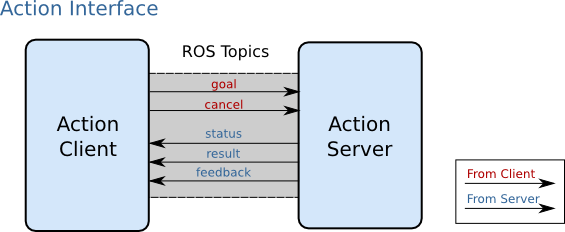
\includegraphics[width=\textwidth]{img/action_interface.png}
    \caption{Client-Server Interaction}
    \label{fig:action_interface}
\end{figure}

The communication messages used in this library is: 
\begin{itemize}
    \item \texttt{goal} - used to send new goals to server.
    \item \texttt{cancel} - used to send cancel requests to server.
    \item \texttt{status} - used to notify clients on the current state of every goal in the system.
    \item \texttt{feedback} - used to send clients periodic auxiliary information for a goal.
    \item \texttt{result} - used to send clients one-time auxiliary information upon completion of a goal.
\end{itemize} 

Action templates are defined by a name and some additional properties through an 
\texttt{*.action} structure defined in ROS. Each instance of an action has a unique 
\textit{Goal ID} which provides the action server and the action client with a robust 
way to monitor the execution of a particular instance of an action.

In our system, its used a \texttt{SimpleActionServer} that implements a single goal policy.
So only one goal can have an active status at a time. When recived new goals preempt previous 
goals based on the stamp in their \textit{Goal ID} field. And a \texttt{SimpleActionClient} which 
implements a simplified \textit{ActionClient}.

As previously mentioned, the \texttt{move\_base} package provides an implementation
of an action that, given a goal in the world, will attempt to reach it with a mobile base.

An example of \texttt{move\_base} \textit{ActionServer}:
\begin{itemize}
    \item {\bf Action Subscribed Topics:}
    \begin{itemize}
        \item \texttt{move\_base/goal} (\textit{move\_base\_msgs/MoveBaseActionGoal}): a goal for \texttt{move\_base} to pursue in the world.
        \item \texttt{move\_base/cancel} (\textit{actionlib\_msgs/GoalID}): a request to cancel a specific goal.
    \end{itemize} 
    \item {\bf Action Published Topics:}
    \begin{itemize}
        \item \texttt{move\_base/feedback} (\textit{move\_base\_msgs/MoveBaseActionFeedback}): feedback contains the current position of the base in the world.
        \item \texttt{move\_base/status} (\textit{actionlib\_msgs/GoalStatusArray}): provides status information on the goals that are sent to the \texttt{move\_base} action.
        \item \texttt{move\_base/result} (\textit{move\_base\_msgs/MoveBaseActionResult}): result is empty for the \texttt{move\_base} action.
    \end{itemize}
\end{itemize}

\subsection{\texttt{task\_planner} package}
We extend the \texttt{patrolling\_sim} package creating a new extern package which 
comunicate with it. 
The \texttt{task\_planner} generate the finite task set, its receive the initialization message 
from each robot and depending on the message start the different algorithm. 
Then this package implements the centralized coordinator and return the \texttt{mission}
for the robots.

\begin{figure} [hbt]
    \centering
    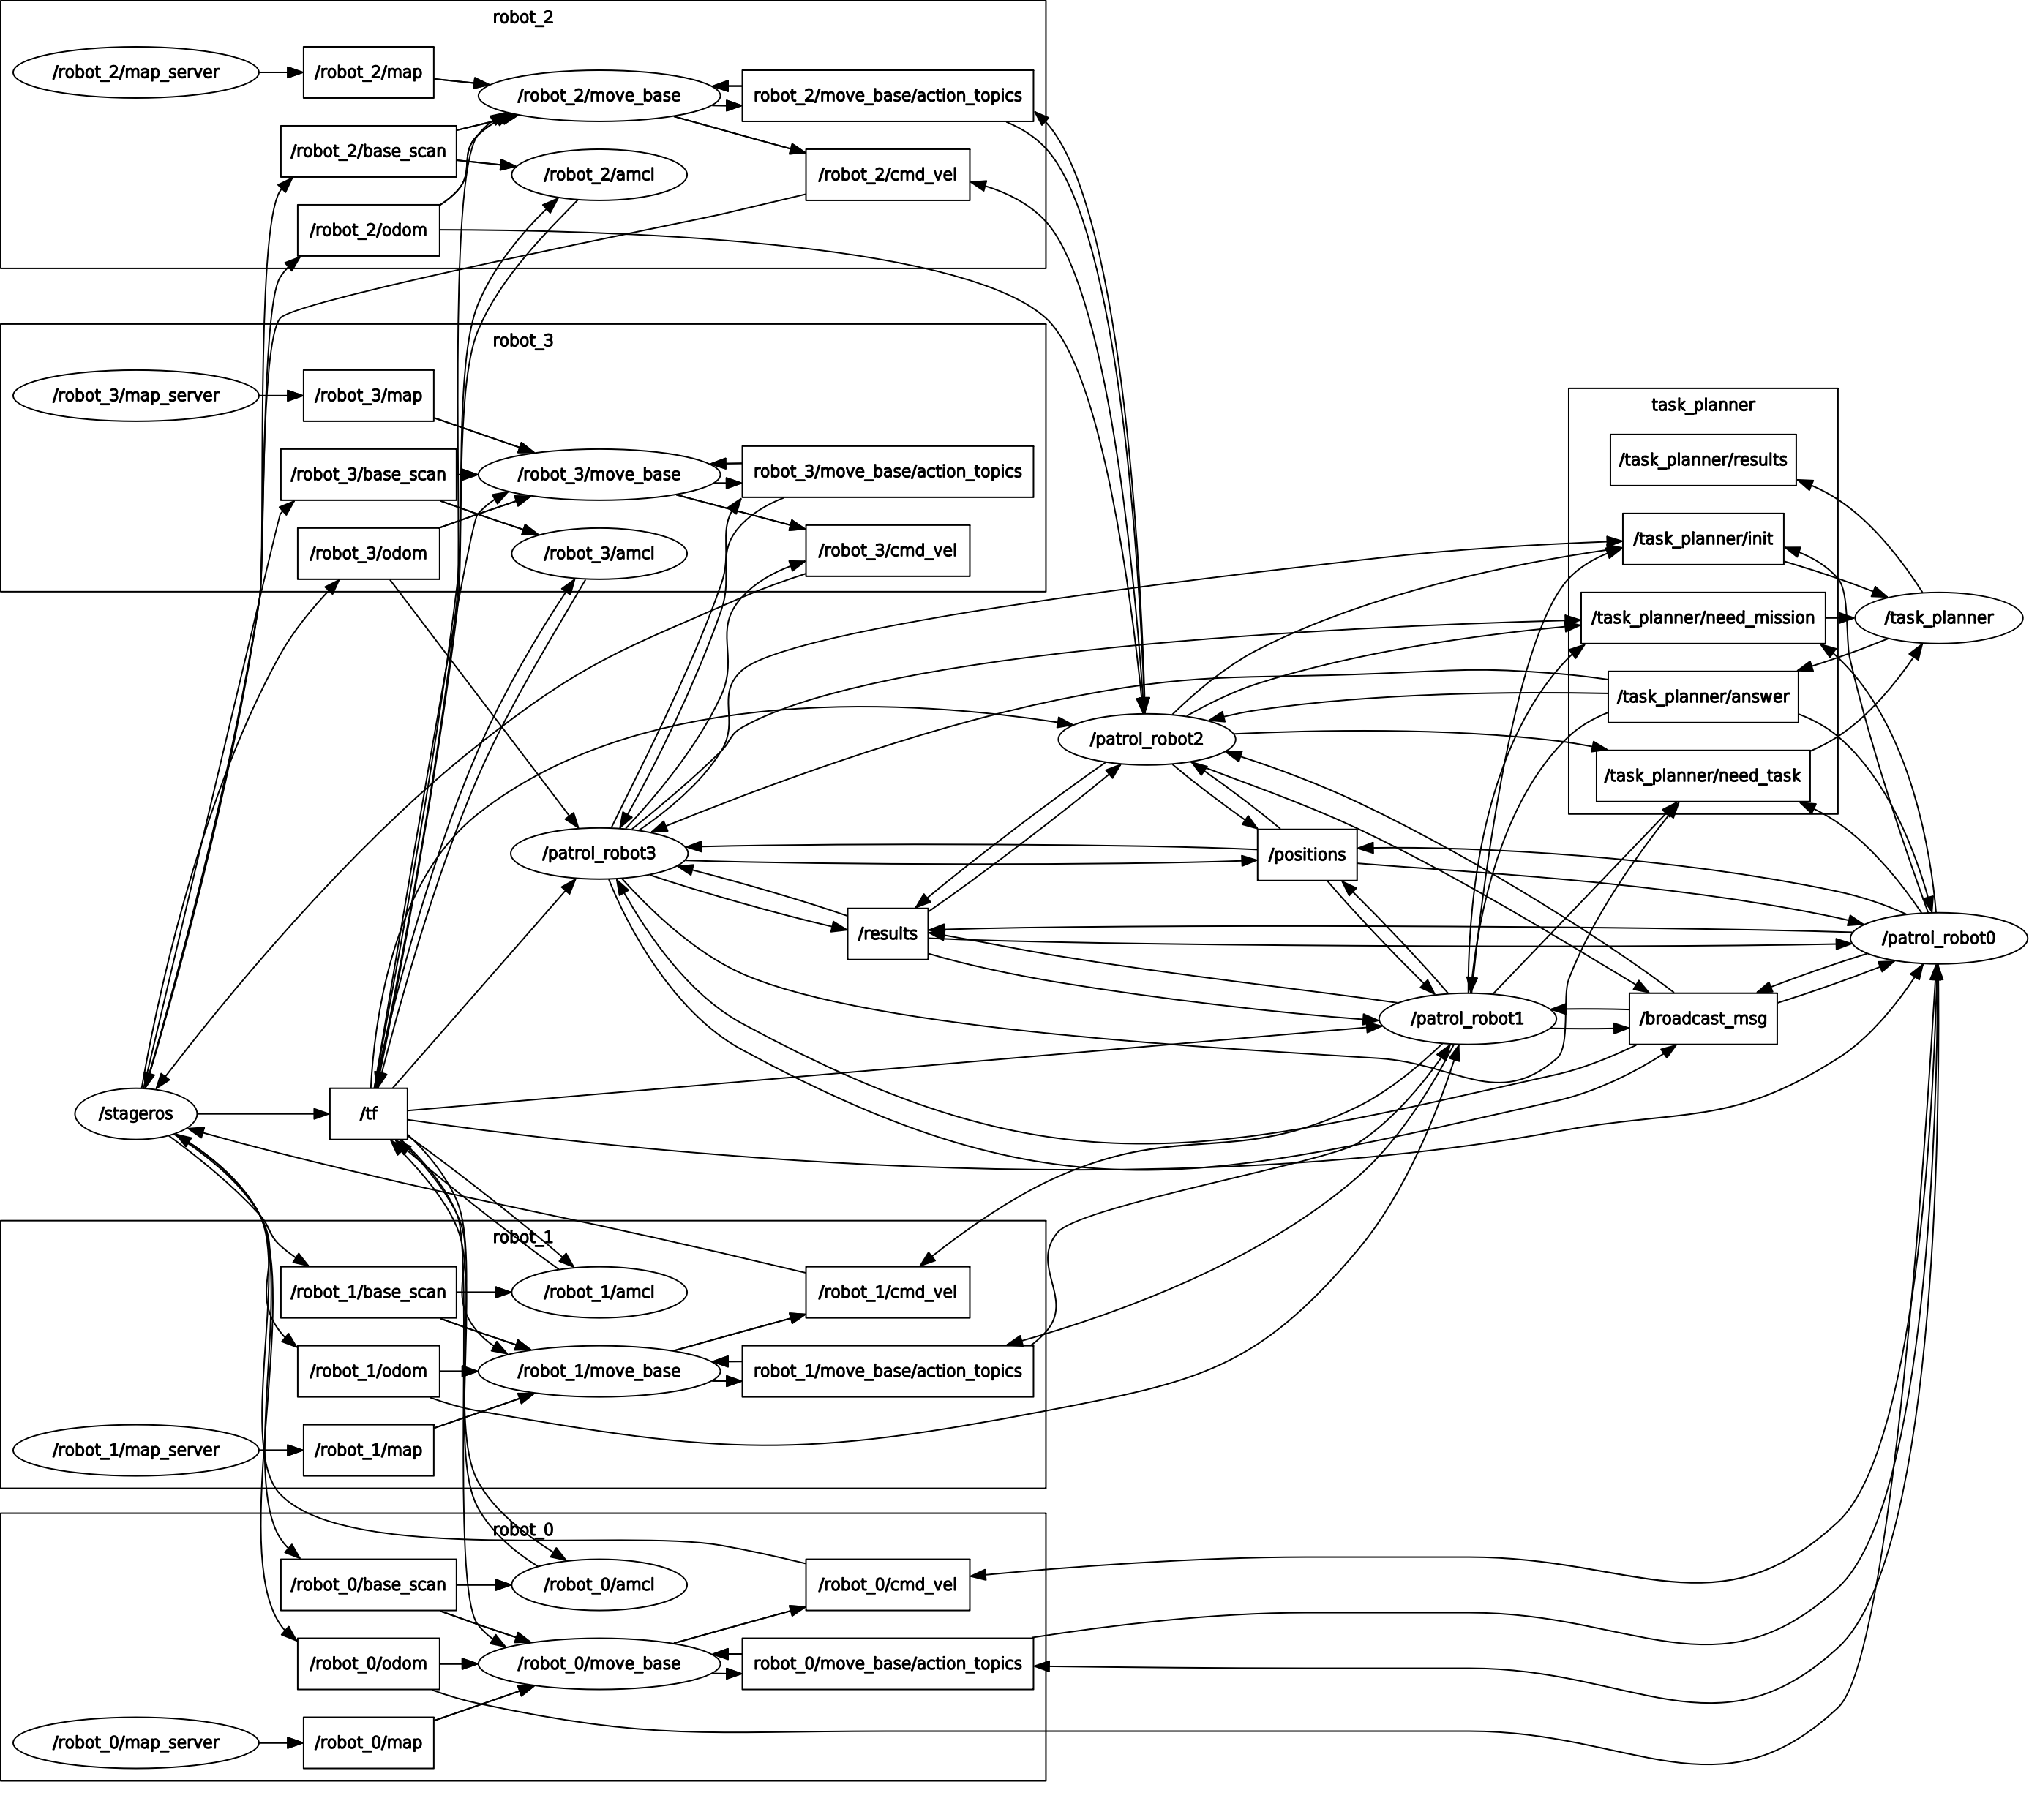
\includegraphics[width=\textwidth]{img/rosgraph.png}
    \caption{Report the \texttt{rqt\_graph}}
    \label{fig:rqt_graph}
\end{figure}

In Figure \ref{fig:rqt_graph} we can see the communication between robots (\texttt{/patrol\_robot}$N$) 
and \texttt{task\_planner}.
\newpage

The most important topisc are:
\begin{itemize}
    \item \texttt{/task\_planner/init}: receive the initialization message.
    \item \texttt{/task\_planner/need\_task}: receive the task request.
    \item \texttt{/task\_planner/need\_mission}: receive the mission request.
    \item \texttt{/task\_planner/answer}: after computation phase for different algorithm return the subset of task must be allocate. 
\end{itemize}












\chapter{Empirical Results}\label{chap:results}
\input{chapter/experiments.tex}


\begin{table}[hbt]
    \centering
    \begin{tabular}{|c|c|c|c|c|c|} \hline
    {\bf Configuration} & {\bf Algorithm} & {\bf $ \overline{Time}$} & {\bf $\overline{Interference}$} & {\bf $\overline{Distance}$} & {\bf $\bar{\sigma}(Distance)$}         \\ \hline
    *6/-/2               & \srst           & 218.32$[\pm 6.19]$        & 63.45   & 3747.90 &  87.8\\ \hline 
    *6/3/2               & \gsp            & 194.52$[\pm 6.42]$        & 49.65    & 3401.15 & 251.37  \\ 
    *                    & \sps            & 177.00$[\pm 1.99]$        & 49.34    & 3132.5 & 0  \\ \hline
    *6/5/2               & \gsp            & 142.08$[\pm 1.39]$       &   42.2        & 2714.25      &  206.43  \\
    *                    & \sps            & 138.98$[\pm 2.41]$       &  39.38   &  2601.25  &  156.47   \\ \hline
    *6/-/4               & \srst           & 124.52$[\pm 3.12]$        & 42    & 2194.75 &  114.2 \\ \hline
    *6/3/4               & \gsp            & 117.44$[\pm 1.85]$        & 35.75   & 1769 & 43.83  \\ 
    *                    & \sps            & 115.28$[\pm 4.10]$        & 33.5   & 1702.5 & 23.67  \\ \hline
    *6/5/4               & \gsp            &  93.4$[\pm 1.01]$         & 29     & 1688.5 &  34.5   \\
    *                     & \sps            &  91.8$[\pm 2.14]$        & 30.75  & 1546.5 & 35.8  \\ \hline
    *9/-/2               & \srst           & 292.24$[\pm 3.06]$      &  85.5  & 5201.5 & 34.76\\ \hline
    *9/3/2              & \gsp            & 265.72$[\pm 2.64]$      & 71.5   & 4491.5  & 0  \\ 
    *                   & \sps            & 240.74$[\pm 10.42]$        & 75.5    & 4232.5 & 310.43 \\ \hline
    * 9/5/2             & \gsp          & 232.84$[\pm 4.71]$      &  68.85  &  4041.25  &  236 \\
    *                   & \sps           &168.34$[\pm 2.03]$       &   50.5   & 3132.5 &  0  \\ \hline 
    *9/-/4               & \srst           & 178.55$[\pm 4.23]$     & 52  & 2755.75 & 135.8 \\ \hline
    *9/3/4               & \gsp            & 152.55$[\pm 2.87]$     & 46.75 & 2200 & 113.4 \\ 
    *                   & \sps            & 134.23$[\pm 3.25]$     &  40.63   & 2182.5 & 27 \\ \hline
    *9/5/4              & \gsp           &134.23$[\pm 3.26]$        & 40.6    & 2098.3     &   93.45    \\
    *                   & \sps           &93.05$[\pm 5.15]$         & 32.25    & 1530.25 &   0 \\ \hline    
    
    *21/-/2             & \srst           & 629.10$[\pm 8.84]$        & 154.6   &11773.5 &  229.75 \\ \hline
    *21/3/2              & \gsp            & 561.93$[\pm 8.00]$     &  134.3  &10133.16 &  201.2   \\ 
    *21/5/2              & \gsp            & 497.45$[\pm 6.15]$      & 126  & 9079 & 210.4  \\ \hline
    *21/-/4              & \srst           & 402.12$[\pm 5.06]$     & 132.25  & 6232.35 &  295.1 \\ \hline
    @21/3/4              & \gsp            &  & &  & -  \\ 
    @21/5/4              & \gsp            &  & &  & -  \\ \hline
   *42/-/2              & \srst           & 1283.2$[\pm 25.27]$     & 336   & 22446.63 &  323.8 \\ \hline
    @42/3/2              & \gsp            & &  &  & -  \\ 
    @42/5/2              & \gsp            & &  &  & -  \\ \hline
    @42/-/4              & \srst           & &  &  &  - \\ \hline
    @42/3/4              & \gsp            & &  &  & -  \\ 
    @42/5/4              & \gsp            & &  &  & -  \\ \hline
\end{tabular}
\end{table}


































\chapter{Conclusions and Future Work}\label{chap:conclusions}
In this thesis we have shown how our system can perform pickup-and-delivery tasks.
We evaluate the performance of our system in a realistic simulation enviroment,
precisely on the ICE Laboratory build with ROS and stage. 
In particular we compared our task assignment approches with the baseline greedy 
approch.

We have discovered that a coalition formation problem can approximate the results 
of a set partion problem in less time complexity.

Because we are focused on a centralized coordinator in the future works we want to 
perform a distributed coordiantor using a recent stategy studied before to implement 
our approaches.
In more detail on \cite{mapd} they used a Token Passing strategy with kinematic 
constraints but consider only one task assigned to one robot at time.
We want to extend this limitations considering the possibility of assigning more 
tasks in one travel.
That strategy should be more flessible, adaptive at the situation on the traveling
orders then fault-tolenace. 

The scope set at the beginning of the thesis have been reached.
The results comfirmed the expectations. 

Then in coclusion the \gsp algorithm aproximate the \sps strategy on the same task set,
calculating the solution in polynomial time complexity.


% \chapter*{Acknowledgements}
% \addcontentsline{toc}{chapter}{\protect\numberline{}Acknowledgements}

\chapter*{Apendices}
\section*{Appendix A} \label{app:A}
\subsection*{ROS: \texttt{amcl} configuration}

\begin{lstlisting}
    <?xml version="1.0" encoding="UTF-8" ?>
    <launch>
    <arg name="robotname" default="robot_0" />
    <node pkg="amcl" type="amcl" name="amcl" args="scan:=base_scan">
      <!-- Publish scans from best pose at a max of 10 Hz -->
      <param name="odom_model_type" value="diff"/>
      <param name="odom_alpha5" value="0.1"/>
      <param name="transform_tolerance" value="0.2" />
      <param name="gui_publish_rate" value="-10.0"/>
      <param name="laser_max_beams" value="30"/>
      <param name="min_particles" value="100"/>
      <param name="max_particles" value="500"/>
      <param name="kld_err" value="0.05"/>
      <param name="kld_z" value="0.99"/>
      <param name="odom_alpha1" value="0.2"/>
      <param name="odom_alpha2" value="0.2"/>
      <!-- translation std dev, m -->
      <param name="odom_alpha3" value="0.8"/>
      <param name="odom_alpha4" value="0.2"/>
      <param name="laser_z_hit" value="0.5"/>
      <param name="laser_z_short" value="0.05"/>
      <param name="laser_z_max" value="0.05"/>
      <param name="laser_z_rand" value="0.5"/>
      <param name="laser_sigma_hit" value="0.2"/>
      <param name="laser_lambda_short" value="0.1"/>
      <param name="laser_lambda_short" value="0.1"/>
      <param name="laser_model_type" value="likelihood_field"/>
      <!-- <param name="laser_model_type" value="beam"/> -->
      <param name="laser_likelihood_max_dist" value="2.0"/>
      <param name="update_min_d" value="0.2"/>
      <param name="update_min_a" value="0.5"/>
      <param name="odom_frame_id" value="odom"/>
      <param name="base_frame_id" value="base_link"/>
      <param name="resample_interval" value="1"/>
    </node>
    </launch>
    \end{lstlisting}
\newpage
\section*{Appendix B} \label{app:B}
% tabelle degli esperimenti ordine SRST GSP SP
\begin{table}[hbt]
    \centering
    \begin{tabular}{|c|c|c|c|} \hline
    {\bf Algorithm} &{\bf Number of task} & {\bf Capacity} & {\bf Time}         \\ \hline
    \srst         & 6              & -       & 218.33      \\ \hline
    {\bf robot}     & {\bf processed task}     & {\bf distance} & {\bf interference} \\ \hline
    0               & 3           & 3739  & 63         \\
    1               & 3              & 3757  & 57       \\ \hline
    \end{tabular}
\end{table}

% \begin{multicols}{2}
\begin{table}[hbt]
    \centering
    \begin{tabular}{|c|c|c|c|} \hline
    {\bf Algorithm} &{\bf Number of task} & {\bf Capacity} & {\bf Time}         \\ \hline
    \gsp            & 6              & 3        & {\bf 194.52}       \\ \hline
    {\bf robot}     & {\bf processed task}     & {\bf distance} & {\bf interference} \\ \hline
    0               & 2              & 3286  & 48        \\
    1               & 2              & 3516  & 51       \\ \hline
    \end{tabular}
\end{table}

\begin{table}[hbt]
    \centering
    \begin{tabular}{|c|c|c|c|} \hline
    {\bf Algorithm} &{\bf Number of task} & {\bf Capacity} & {\bf Time}         \\ \hline
    \sps          & 6              & 3        & 177      \\ \hline
    {\bf robot}     & {\bf processed task}     & {\bf distance} & {\bf interference} \\ \hline
    0               & 2              & 2970 & 47       \\
    1               & 2              & 3295  & 52        \\ \hline
    \end{tabular}
\end{table}

% \end{multicols}

\begin{table}[hbt]
    \centering
    \begin{tabular}{|c|c|c|c|} \hline
    {\bf Algorithm} &{\bf Number of task} & {\bf Capacity} & {\bf Time}         \\ \hline
    \gsp            & 6              & 5        & 142       \\ \hline
    {\bf robot}     & {\bf processed task}     & {\bf distance} & {\bf interference} \\ \hline
    0               & 2              & 3074  & 47       \\
    1               & 1             & 2355  & 38       \\ \hline
    \end{tabular}
\end{table}

\begin{table}[hbt]
    \centering
    \begin{tabular}{|c|c|c|c|} \hline
    {\bf Algorithm} &{\bf Number of task} & {\bf Capacity} & {\bf Time}         \\ \hline
    \sps          & 6              & 5        &  138.98     \\ \hline
    {\bf robot}     & {\bf processed task}     & {\bf distance} & {\bf interference} \\ \hline
    0               & 2              & 2847  & 43      \\
    1               & 1             &  2355 & 35       \\ \hline
    \end{tabular}
\end{table}

% stesso setup ma con 4 robot

\begin{table}[hbt]
    \centering
    \begin{tabular}{|c|c|c|c|} \hline
    {\bf Algorithm} &{\bf Number of task} & {\bf Capacity} & {\bf Time}         \\ \hline
    \srst         & 6              & -      & 124.52      \\ \hline
    {\bf robot}     & {\bf processed task}     & {\bf distance} & {\bf interference} \\ \hline
    0               & 2         & 2060  & 31         \\
    1               & 2         & 2337  & 59         \\
    2               & 1         & 2434  & 38         \\
    3               & 1         & 1949  & 40         \\ \hline
    \end{tabular}
\end{table}

\begin{table}[hbt]
    \centering
    \begin{tabular}{|c|c|c|c|} \hline
    {\bf Algorithm} &{\bf Number of task} & {\bf Capacity} & {\bf Time}         \\ \hline
    \gsp       & 6              & 3        & 117.44      \\ \hline
    {\bf robot}     & {\bf processed task}     & {\bf distance} & {\bf interference} \\ \hline
    0               & 1         & 1860  & 32        \\
    1               & 1         & 1853 & 31         \\
    2               & 1         & 1675  & 40       \\
    3               & 1         & 1688 & 40        \\ \hline
    \end{tabular}
\end{table}

\begin{table}[hbt]
    \centering
    \begin{tabular}{|c|c|c|c|} \hline
    {\bf Algorithm} &{\bf Number of task} & {\bf Capacity} & {\bf Time}         \\ \hline
    \sps      & 6              & 3        & {\bf 115.28}     \\ \hline
    {\bf robot}     & {\bf processed task}     & {\bf distance} & {\bf interference} \\ \hline
    0               & 1         & 1897 & 30    \\
    1               & 1         & 1854  & 37        \\
    2               & 1         & 1647 & 35      \\
    3               & 1         & 1412 & 32      \\ \hline
    \end{tabular}
\end{table}

\begin{table}[hbt]
    \centering
    \begin{tabular}{|c|c|c|c|} \hline
    {\bf Algorithm} &{\bf Number of task} & {\bf Capacity} & {\bf Time}         \\ \hline
    \gsp       & 6              & 5        & 93.4     \\ \hline
    {\bf robot}     & {\bf processed task}     & {\bf distance} & {\bf interference} \\ \hline
    0               & 1         & 1753  & 32       \\
    1               & 1         & 1960 & 35         \\
    2               & 1         & 2414  & 34      \\
    3               & {\bf 0}   & (627) & (15)        \\ \hline
    \end{tabular}
\end{table}

\begin{table}[hbt]
    \centering
    \begin{tabular}{|c|c|c|c|} \hline
    {\bf Algorithm} &{\bf Number of task} & {\bf Capacity} & {\bf Time}         \\ \hline
    \sps      & 6              & 5       & {\bf 91.8}     \\ \hline
    {\bf robot}     & {\bf processed task}     & {\bf distance} & {\bf interference} \\ \hline
    0               & 1         & 1105 & 29    \\
    1               & 1         & 2407  & 37        \\
    2               & 1         & 1959 & 33      \\
    3               & {\bf 0}   & (715) & (24)     \\ \hline
    \end{tabular}
\end{table}

% --------
\begin{table}[hbt]
    \centering
    \begin{tabular}{|c|c|c|c|} \hline
    {\bf Algorithm} &{\bf Number of task} & {\bf Capacity} & {\bf Time}         \\ \hline
    \srst         & 9              & -       & 292.24      \\ \hline
    {\bf robot}     & {\bf processed task}     & {\bf distance} & {\bf interference} \\ \hline
    0         & 5              & 5631  & 93       \\ 
    1               & 4         & 4772  & 78         \\\hline
    \end{tabular}
\end{table}

\begin{table}[hbt]
    \centering
    \begin{tabular}{|c|c|c|c|} \hline
        {\bf Algorithm} &{\bf Number of task} & {\bf Capacity} & {\bf Time}         \\ \hline
        \gsp            & 9              & 3        & 265.72       \\ \hline
        {\bf robot}     & {\bf processed task}     & {\bf distance} & {\bf interference} \\ \hline
        0               & 3             & 4578  & 69        \\
        1               & 3              & 4405  & 74       \\ \hline
    \end{tabular}
\end{table}

\begin{table}[hbt]
    \centering
    \begin{tabular}{|c|c|c|c|} \hline
        {\bf Algorithm} &{\bf Number of task} & {\bf Capacity} & {\bf Time}         \\ \hline
        \sps          & 9              & 3        &  240.74      \\ \hline
        {\bf robot}     & {\bf processed task}     & {\bf distance} & {\bf interference} \\ \hline
        0               & 3              & 4412  & 79        \\
        1               & 3              & 4571  & 82        \\ \hline
    \end{tabular}
\end{table}

% ----> 9 task 4 robot C = 3
\begin{table}[hbt]
    \centering
    \begin{tabular}{|c|c|c|c|} \hline
        {\bf Algorithm} &{\bf Number of task} & {\bf Capacity} & {\bf Time}         \\ \hline
        \gsp            & 9              & 5        & 232.84      \\ \hline
        {\bf robot}     & {\bf processed task}     & {\bf distance} & {\bf interference} \\ \hline
        0               & 3            & 4207  & 71    \\
        1               & 3              & 3875  & 67       \\ \hline
    \end{tabular}
\end{table}


\begin{table}[hbt]
    \centering
    \begin{tabular}{|c|c|c|c|} \hline
    {\bf Algorithm} &{\bf Number of task} & {\bf Capacity} & {\bf Time}         \\ \hline
    \sps          & 9              & 5        & {\bf 168.34}      \\ \hline
    {\bf robot}     & {\bf processed task}     & {\bf distance} & {\bf interference} \\ \hline
    0               & 2             & 2970  & 45      \\
    1               & 2              & 3295 & 56       \\ \hline
    \end{tabular}
\end{table}

\begin{table}[hbt]
    \centering
    \begin{tabular}{|c|c|c|c|} \hline
    {\bf Algorithm} &{\bf Number of task} & {\bf Capacity} & {\bf Time}         \\ \hline
    \srst       & 9             & -        & 178.55      \\ \hline
    {\bf robot}     & {\bf processed task}     & {\bf distance} & {\bf interference} \\ \hline
    0               & 3        & 3582  & 64       \\
    1               & 3         & 2833 & 55    \\
    2               & 2       & 2635  & 46   \\
    3               & 1        & 1973 &  43    \\ \hline
    \end{tabular}
\end{table}

\begin{table}[hbt]
    \centering
    \begin{tabular}{|c|c|c|c|} \hline
    {\bf Algorithm} &{\bf Number of task} & {\bf Capacity} & {\bf Time}         \\ \hline
    \gsp       & 9             & 3        & 152.55      \\ \hline
    {\bf robot}     & {\bf processed task}     & {\bf distance} & {\bf interference} \\ \hline
    0               & 2         & 2921  & 61       \\
    1               & 2         & 2167 & 49    \\
    2               & 1        & 1994  & 39     \\
    3               & 1         & 1718 &  38    \\ \hline
    \end{tabular}
\end{table}

\begin{table}[hbt]
    \centering
    \begin{tabular}{|c|c|c|c|} \hline
    {\bf Algorithm} &{\bf Number of task} & {\bf Capacity} & {\bf Time}         \\ \hline
    \sps    & 9             & 3        & 134.23      \\ \hline
    {\bf robot}     & {\bf processed task}     & {\bf distance} & {\bf interference} \\ \hline
    0               & 2         & 2826  & 52       \\
    1               & 1        & 1960 & 35     \\
    2               & 1       & 2135 & 39   \\
    3               & 1         & 1809 & 36       \\ \hline
    \end{tabular}
\end{table}


% c=5 9 task

\begin{table}[hbt]
    \centering
    \begin{tabular}{|c|c|c|c|} \hline
    {\bf Algorithm} &{\bf Number of task} & {\bf Capacity} & {\bf Time}         \\ \hline
    \gsp       & 9             & 5       & 134.23     \\ \hline
    {\bf robot}     & {\bf processed task}     & {\bf distance} & {\bf interference} \\ \hline
    0               & 2         & 2785 & 52       \\
    1               & 1        & 1960 & 35    \\
    2               & 1        & 2135  & 39     \\
    3               & 1         & 1514 &  36    \\ \hline
    \end{tabular}
\end{table}

\begin{table}[hbt]
    \centering
    \begin{tabular}{|c|c|c|c|} \hline
    {\bf Algorithm} &{\bf Number of task} & {\bf Capacity} & {\bf Time}         \\ \hline
    \sps      & 9             & 5       & {\bf 93.05}     \\ \hline
    {\bf robot}     & {\bf processed task}     & {\bf distance} & {\bf interference} \\ \hline
    0               & 2        & 1374 & 42       \\
    1               & 1        & 2067 & 35    \\
    2               & 1        & 2054  & 36     \\
    3               & {\bf 0}        & (626) &  (16)    \\ \hline
    \end{tabular}
\end{table}


\begin{table}[hbt]
    \centering
    \begin{tabular}{|c|c|c|c|} \hline
    {\bf Algorithm} &{\bf Number of task} & {\bf Capacity} & {\bf Time}         \\ \hline
    \srst       & 21            & -        & 629      \\ \hline
    {\bf robot}     & {\bf processed task}     & {\bf distance} & {\bf interference} \\ \hline
    0               & 11       & 12091  & 165       \\
    1               & 10        & 11456 & 145    \\ \hline
    \end{tabular}
\end{table}

\begin{table}[hbt]
    \centering
    \begin{tabular}{|c|c|c|c|} \hline
    {\bf Algorithm} &{\bf Number of task} & {\bf Capacity} & {\bf Time}         \\ \hline
     \gsp      & 21            & 3      & 561.93      \\ \hline
    {\bf robot}     & {\bf processed task}     & {\bf distance} & {\bf interference} \\ \hline
    0               & 7       & 9943 & 130      \\
    1               & 7        & 10323 & 139   \\ \hline
    \end{tabular}
\end{table}

\begin{table}[hbt]
    \centering
    \begin{tabular}{|c|c|c|c|} \hline
    {\bf Algorithm} &{\bf Number of task} & {\bf Capacity} & {\bf Time}         \\ \hline
    \gsp      & 21            & 5     & 497.45      \\ \hline
    {\bf robot}     & {\bf processed task}     & {\bf distance} & {\bf interference} \\ \hline
    0               & 6     & 8816  & 115       \\
    1               & 6     & 9343 & 137    \\ \hline
    \end{tabular}
\end{table}

\begin{table}[hbt]
    \centering
    \begin{tabular}{|c|c|c|c|} \hline
    {\bf Algorithm} &{\bf Number of task} & {\bf Capacity} & {\bf Time}         \\ \hline
    \srst         & 21              & -      & 402      \\ \hline
    {\bf robot}     & {\bf processed task}     & {\bf distance} & {\bf interference} \\ \hline
    0               & 6        & 7069 & 152       \\
    1               & 5         & 5731  & 119         \\
    2               & 5         & 5928  & 109        \\
    3               & 5         & 6201  & 129        \\ \hline
    \end{tabular}
\end{table}

\begin{table}[hbt]
    \centering
    \begin{tabular}{|c|c|c|c|} \hline
    {\bf Algorithm} &{\bf Number of task} & {\bf Capacity} & {\bf Time}         \\ \hline
    \gsp         & 21              & 3     & 343.23     \\ \hline
    {\bf robot}     & {\bf processed task}     & {\bf distance} & {\bf interference} \\ \hline
    0               & 4         & 6134 & 97      \\
    1               & 4         & 5731  & 103         \\
    2               & 3         & 5452  & 95        \\
    3               & 3         & 4201  & 85        \\ \hline
    \end{tabular}
\end{table}

\begin{table}[hbt]
    \centering
    \begin{tabular}{|c|c|c|c|} \hline
    {\bf Algorithm} &{\bf Number of task} & {\bf Capacity} & {\bf Time}         \\ \hline
    \gsp         & 21              & 5     & 294.4     \\ \hline
    {\bf robot}     & {\bf processed task}     & {\bf distance} & {\bf interference} \\ \hline
    0               & 3       & 4905 & 83       \\
    1               & 3         & 5455  & 72         \\
    2               & 3         & 4146  & 82        \\
    3               & 3         & 4227  & 75        \\ \hline
    \end{tabular}
\end{table}


\begin{table}[hbt]
    \centering
    \begin{tabular}{|c|c|c|c|} \hline
    {\bf Algorithm} &{\bf Number of task} & {\bf Capacity} & {\bf Time}         \\ \hline
    \srst       & 42           & -        & 1283.2     \\ \hline
    {\bf robot}     & {\bf processed task}     & {\bf distance} & {\bf interference} \\ \hline
    0               & 21       & 22243  & 335      \\
    1               & 21       & 22651 & 338    \\ \hline
    \end{tabular}
\end{table}



% \chapter*{Bibliography}
\begin{thebibliography}{99}
    \bibitem{parker} L.E. Parker, 
    \emph{Distributed Intelligence: Overview of the Field and its
    Application in Multi-Robot Systems}, March 2008.

    \bibitem{maxsum} A. Farinelli, N. Boscolo, E. Zanotto, E. Pagello,
    \emph{Advanced Approaches for Multi-Robot Coordination in
    Logistic Scenarios}, April 2017.

    \bibitem{mapd} H. Ma, W. Hönig, T.K.S. Kumar, N. Ayanian, S. Koenig,
    \emph{Lifelong Path Planning with Kinematic Constraints
    for Multi-Agent Pickup and Delivery}, December 2018.

    \bibitem{cooros} T. Andre, D. Neuhold, C. Bettstetter,
    \emph{Coordinated Multi-Robot Exploration:
    Out of the Box Packages for ROS}, December 2014.

    \bibitem{cf_farinelli} A. Farinelli, M. Bicego, F. Bistaffa, S. D. Ramchurn,
    \emph{A Hierarchical Clustering Approach to Large-scale
    Near-optimal Coalition Formation with Quality
    Guarantees}, March 2017.

    \bibitem{cf_greedy} X. Zheng, S. Koenig,
    \emph{Greedy Approaches for Solving Task-Allocation Problems with Coalitions}
    , 2008.

    \bibitem{partition} M. Orlov,
    \emph{Efficient Generation of Set Partitions}, March 2002.

    \bibitem{farinelli_coo} A. Farinelli, L. Iocchi, D. Nardi,
    \emph{Multirobot Systems: A Classification
    Focused on Coordination}, October 2004.

    \bibitem{market-based} R. Zlot, A. Stentz, 
    \emph{Market-based Multirobot Coordination for Complex Tasks}, January 2006.

    \bibitem{mapf} H. MA, J. Li, T. K. S. Kumar, S. Koenig,
    \emph{Lifelong Multi-Agent Path Finding
    for Online Pickup and Delivery Tasks}, May 2017.

    \bibitem{decoo} R. Stranders, A. Farinelli, A. Rogers, N. R. Jennings,
    \emph{Decentralised Coordination of Mobile Sensors Using the Max-Sum Algorithm}, 2009.

    \bibitem{focoo} A. Farinelli, L. Iocchi, D. Nardi,
    \emph{Multirobot Systems: A Classification
    Focused on Coordination}, October 2004.

    \bibitem{autocoo}, C. Jones, M. J. Mataric,
    \emph{Automatic Synthesis of Communication-Based
    Coordinated Multi-Robot Systems}, October 2004.

    \bibitem{coocoo}, P. R. Wurman, R. D'AndreA, M. Mountz,
    \emph{Coordinating Hundreds of
    Cooperative, Autonomous
    Vehicles in Warehouses}, March 2008.
    
    
\end{thebibliography} 

% \bibliographystyle{splncs03}
% \bibliography{biblio}

\end{document}
